%\documentstyle[11pt]{article}
\documentclass[11pt]{article}

\usepackage{graphicx}

\input{epsf}
\voffset -1.0cm    
\hoffset -2.0cm     
\textheight 24.0cm
\textwidth 16cm
\topmargin 0.0cm
\topskip 0.0cm
\def\fett #1{{\bf #1}}
%\newfont{\sss}{cmssbx10 scaled 1000}
\begin{document}

\thispagestyle{empty}

\begin{center}
{\bf {\huge The  Screened KKR Package\\
Manual (version 1.2)}} \\
\vspace{2cm}

%\begin{figure}[h]
%\begin{center}
%\includegraphics[scale=1.2]{cover.ps}
%\begin{minipage}{17cm}
%\epsfxsize=16cm \epsfysize=16cm {\epsfbox{Sibonds.ps}}
%\end{minipage}
%\end{center}
%\label{fig3}
%\end{figure}
\vspace{2cm}
{\bf \huge Nikos Papanikolaou, March 2002.}
\end{center}


\newpage
\ \\
\tableofcontents 
\ \\
\newpage

\section{Description and General Features}

The Screened or Tight-Binding KKR method can be used to perform 
all electron, electronic
structure  calculations using density functional theory. The
method is based on multiple scattering theory and the Kohn-Sham equations for
a solid are solved by dividing space in cells  and connecting the scattering
events from each individual cell using Green's function formalism (Dyson
equation). You can find general references about the method in the end of this
manual. 

The present package consists of three main programs, the {\tt voronoi, skkr,}
and {\tt impurity}. This give you a rather powerful combination for
electronic structure calculations of solids. The programs can be used for
the calculation of 3D periodic systems, and supercells, 2D finite slabs 
or 2D semiinfinite systems. Impurities can be embedded in any of the
above environments, using the {\tt impurity} program. The Atomic 
Sphere Approximation (ASA) but with full charge density or Full potential 
(FP) calculations are possible. The current version can use simple non
relativistic or scalar relativistic formalism. The TB-formulation of the 
KKR theory allows fast and accurate O(N) scaling calculations for ASA
or FP.    
In the FP space is divide into cells with  a
Wigner-Seitz construction or more general Voronoi construction.  This space
division, potential preparation and lattice analysis
can be done with the {\tt voronoi} program.
Usually for Density of states, bandstructures, 
rough estimates of energetics, magnetic moments, etc ASA is
enough. For better energies, forces (geometry optimizations,
relaxations) full potential has to be used.
Defects in bulk, surfaces, interfaces, including energetics etc.
can be studied with the {\tt impurity} program.

\section{Basic Theory}
% --------------- new part of theory
A central concept in the KKR Green's function method is the use of the Dyson
equation
\begin{equation}
\mathbf{G} = \mathbf{G}^r + \mathbf{G}^r \Delta V \mathbf{G}
\label{dyson1}
\end{equation}
to connect the Green's functions of the true physical system $\mathbf{G}$,
with an arbitrary chosen reference system described by $\mathbf{G}^r$, which
have a difference in the potential $\mathbf \Delta V$. The idea of the
screened KKR is the construction of a reference system for which the Green�s
function decays exponentially in real space. This would lead to short ranged
interactions limited to neighbouring atoms only. For this purpose we use a
lattice of strongly repulsive muffin-tin potentials. This way we can
accomplish screening and thus a tight-binding, band diagonal, form for the
structural Green's function matrix by virtue of the reference system. The true
physical system is not required to have short range interactions. The KKR and
Screened KKR methods and their properties are described in detail 
\cite{kkr1,kkr2,kkr3,kkr6,kkr4,kkr5,kkrgen1,fermidir,fullpot,drittler,kkr0}
\cite{kkr_mrs}, \cite{wildberger} and in references therein. 
Here we will briefly discuss the application
of the SKKR to layered structures and semiinfinite systems, the case of
3D bulk systems is similar, the only difference is that the 2D Fourier
transform has to be replaced by a 3D Fourier transform.  

The Green's function is expressed in the usual cite-centered 
angular momentum expansion
\begin{eqnarray}
\label{podloucky}
 G(\fett r + \fett R_n , \fett r'+ \fett R_{n'} ;E ) =  \delta_{nn'}\, G^n_s
 (\fett r + \fett R_{n}, \fett r' + \fett R_{n'} ;E )
%\nonumber \\[0.4cm]
 { + \, \sum_{L,L'} R^n_L (\fett r ;E ) \, G^{nn'}_{LL'}(E ) \,
R^{n'}_{L'}(\fett r' ;E )}
\end{eqnarray}
where $G^n_s$ is the Green function for a single scattering potential in cell
$n$ in an otherwise free space. Multiple scattering contributions are
contained in the second term through the so-called structural Green function
$G^{nn'}_{LL'}(E)$.  The index $L$ denotes the angular momentum indices
$(l,m)$ and $R^{n}_{L}(\fett r;E)$ are regular partial-wave solutions of the
Schr\"odinger equation for the potential $V^n(\fett r)$ and energy $E$.
 
For layered systems  we apply a 2D-Fourier transform \cite{wildberger}:
\begin{equation}
G_{LL'}^{r \; ii'} (\fett{q}_\parallel ; E ) = \sum_{\nu'} e^{-i
 \fett{q}_\parallel (\fett{\chi}_\nu - \fett{\chi}_{\nu'} )} \;  G_{LL'}^{r \;
 ii' \; \nu - \nu' }(E )
\end{equation}
with the 2D wave vector $\fett{q}_\parallel$, and $\fett\chi_\nu$ are 2D
lattice vectors.  Then the Dyson equation takes the form:
 
\begin{equation}
G_{LL'}^{ii'} (\fett{q}_\parallel ; E ) = G_{LL'}^{r \; ii'}
(\fett{q}_\parallel ; E ) + \sum_{i'' L''} G_{LL''}^{r \; ii''}
(\fett{q}_\parallel ; E ) \; \Delta t_{l''}^{i''} (E) \; G_{L''L'}^{i''i'}
(\fett{q}_\parallel ; E )
\label{dyson_2d}
\end{equation}
where $i$ and $\nu$ denotes  the layer index and  the index for the atomic
site in the layer respectively.  $  \Delta t^{n}_{l} (E)$ is the difference in
the scattering t-matrix between the true and the reference system. The
$t$-matrix is obtained through:
\[ t^{n}_l (E) = \int^{R_{c}}_{0}\;  dr \,r^2 \;  j_l(\sqrt{E}r) \;V^n(r)\; 
R^n_l(r;E), \]
where $j_l(\sqrt{E}r)$ are spherical Bessel functions, and $R_c$ denotes the
muffin-tin sphere (or ASA sphere when the Atomic Sphere Approximation is
used). We consider here only spherical potentials but the extension to
non-spherical, full potential, is straightforward.
 
The calculation of the Green's function requires a matrix inversion. To
simplify the formulas we drop all angular momentum and cite indices. Equation
\ref{dyson_2d} can be easily transformed to:
\begin{equation}
G = \Delta t^{-1} - \Delta t^{-1} \tau \Delta t^{-1}
\label{green1}
\end{equation}
where
\begin{equation}
\tau = (G^r - \Delta t^{-1})^{-1}
\label{green2}
\end{equation}
 
Due to the exponential decrease of the screened structure constants, the
coupling can be limited to few neighbouring shells, so that the 2D Fourier
transform of the reference Green's function has the structure of a band matrix
coupling only neighbouring layers.  Therefore, one can simplify the matrix
$G^{r, ii'}$ by grouping several atomic layers into so-called {\it principal
layers} \cite{decimation,decimation2}, the coupling of which is limited to the
first nearest principal layers only.  Assuming a system of identical repulsive
potentials in a lattice, the reference Green's function has the form:
\begin{equation}
G^{r \;\alpha \beta}  = G^{r \; 00} \delta_{\alpha, \beta} + G^{r \; 01}
\delta_{\alpha ,\beta-1}+ G^{r \; 10} \delta_{\alpha ,\beta+1}
\label{princ}
\end{equation}
where $\alpha, \beta$ are principal layer indices.
 
For the case of a finite slab system the $G^r$ has a finite rank, is band
diagonal and has the form of eq. \ref{princ}, while $\Delta t^{-1}$  is
diagonal in the cite index and in the principal layer representation
eq.\ref{dyson_2d} has the form of the Dyson equation for a linear chain with
nearest neighbour coupling only.  For such systems, the diagonal blocks of the
real system Green�s function $G^{nn}$, which are required to obtain the charge
density, $n(\fett r; E) = -\frac{1}{\pi}ImTrG(\fett r, \fett r;E)$ can be
calculated \cite{godfrin}, \cite{wu} with efford that scales linear with the
number of principal layers in the slab $N$. This $N$-scaling behaviour is one
of the main advantages of the screened KKR approach.
 
The band diagonal form of the Green's function allows us to treat also
semiinfinite systems.  In this case we need to invert an infinite matrix. We
can divide the system in three regions: an  intermediate region (I), embedded
into two (unperturbed) semi-infinite left (L) and right (R) halfspaces. The
regions R and L are characterized by bulk potentials, so that the new
selfconsistency process affects only the potentials of the  region I. 
 Using an inversion-by-partitioning
tequnique it is easy to see that, embedding region I into the semiinfinite L
and R host media would only affect the $G^{11}$ and $G^{NN}$ blocks of the
Green's function matrix. This embedding information is included in the surface
Green's function $G^{11}_{surf}$ (left halfspace), $G^{NN}_{surf}$ (right
halfspace) which we obtain using an iterative procedure, the so called
decimation method, as described in ref \cite{decimation,decimation2}. 
Usually 5-6 iterations are enough, to obtain well converged 
surface Green's functions.
Only a few $\fett{q}_\parallel$ points (i.e. close to Van Hove singularities)
require additional effort.

%----------------------------------------------------------------------------
%----------------------------------------------------------------------------
\section{Technical details}
\subsection{General considerations and philosophy}
The current version of the code implements a screened KKR method. The
traditional KKR method used free space as a reference system and the Green's
function of the true system was found through a Dyson equation. However the
free space structure constants do not converge easily and an Ewald procedure
is necessary for 3D, while Kambe sums are needed for 2D
geometries. This  makes the method complicated and time consuming.  The
screened KKR avoids these problems by introducing a fictitious reference
system of an infinite array of repulsive MT potentials  typically 4 Rydberg 
high. 
Since the structure constants decay exponentially only
a cluster of repulsive MT potentials around each cite is needed. 
{\bf This is often
called the Tight Binding-cluster (TB-cluster). Important is that this
reference system is strictly Muffin-Tin (no overlap) but this has no
limitation on the true system which can be ASA or FP. }

The introduction of the TB-structure constants has at least two big
advantages. First it leads to a banded matrix in the Dyson equation which can
be inverted O(N) for N cites.  The second big advantage is
that the structure constant part of the KKR calculation is simplified and is
unique in 3D, 2D, and even 1D or a real space formulation where a free cluster
is considered with no periodicity.

The current SKKR implementation can treat 3D periodic lattices or super-cells
and multi-layers, and 2D structures where no periodicity is required in the
third direction, like finite slabs or semi-infinite systems using the
"decimation method".

Another advantage of the Green's function formalism is the ability to describe
non periodic  systems like impurities in bulk or surfaces or interfaces
etc. This is done with the  impurity programs which are also included in this
manual. But we will cover the  calculation of "host Green function" briefly
later.

\subsection{Input files}

To perform  a calculation there are a few initial files that are needed. 
{\it The  philosophy is that you need ONLY ONE INPUTFILE called {\tt 
inputcard} 
that contains all the information on the system.} In
the inputcard we also declare the names of the other initial files. 
Usually these files are also calculated by the SKKR package but should be used
as input for further calculations. The file
I12 normally named {\tt 4Ryshift} contains the information for the repulsive
potential used for the screening, a small utility is used to create this file,
and will be removed in the near future. The file I13 has the initial potential 
to
start the calculation. The program stores the potential during iterations 
in a file called {\tt potio}, this file contains the converged potential
after selfconsistency is reached.
The file I40 named usually madelung is obsolete. The file I19 contains
the shape function for the full-potential calculations and is not used for the
ASA calculations, it is created using the kkr programs and it's creation and
use will be explained later.

The file I25, usually named as scoef is used only for the impurity
calculations, and contains the positions of the atoms for which a Green's
function should be calculated. The file that  is always named "lebedev"
contains the information about integration over a sphere. In particular it is
a special angular mesh that has cubic symmetry and is used to produce Gaunt
coefficients that do not brake the cubic symmetry, so {\bf lebedev should
never be changed.} Finally  we need  also to create a directory called
{\tt mesh\ } where the program will go in and write the k-points file.  Having 
all
these files we can run a calculation.


The explanation of the input parameters can be found in the end of the  manual
here we give a step-by-step guide to start a small calculation.  In the
examples at the end of this manual you can find the setup for  different
simple systems like bulk bcc Fe and for different slabs, supercells and a more
complicated Fe/ZnSe/Fe interface which demonstrates the decimation method.
Then we will mention some practical problems that someone should  have in mind
when doing calculations, the parameters used to compile the KKR code,
the decimation technique,  and how to produce the BAND STRUCTURE, DOS and the
Q-DOS, green function for impurities etc.

\section{Step by step Cu bulk, ASA, self-consistency, dos and band structure}

We start by preparing an inputcard file Use OPTION 'full inv'. Set the
ALATBASIS=6.76d0, LMAX=3, NATYP=1,  the BRAVAIS vectors for
fcc, RBASIS is the zero vector, INTERFACE=.FALSE. since we are doing a 3d
calculation, RCLUSTZ, RCLUSTXY should be set the same, a bigger value
increases the size of the TB-cluster  thus increasing computer time. A value
1.1 should be ok for this test (first and second neighbors).  ATOMINFO
needs the atomic number say 29.00
for Cu, the core configuration,  1  3 3 0 0, for 1s,2s,3s,2p,3p core CLS is 1,
REFPOT is also 1, NTC is 1, IRNS is 1 if ASA and is usually set to 278 for FP.
RMT plays no role in ASA but
should be set correctly for Full potential, the program {\tt voronoi} helps to
decide on this. WEIGHT is usually set to 1.0 but if the basis has more than
one atoms then it could be  set to a different value. The bigger the weight the
bigger the cell of the atom.

After this we need an energy contour for the valence integration, the
{\tt voronoi} program helps to decide where to start the energy 
contour which ends
usually at the Fermi level. A rectangular contour in used with temperature so
usual values are EMIN=-0.4 the correct value depends on the system and 
is suggested by the {\tt voronoi} program. EMAX=1.d0,
this value is usually ignored during self consistency, the EMAX that apears in
the potential is used instead. EMAX is used  in case of DOS calculation.
NPOL=5 (usually), NPT1=3, NPT2=20, NPT3=3, are typical values. 
The number of points for BZ
integration BZDIVIDE= 30    30     30 (for x,y,z directions). Then we have the
self consistency parameters, the filenames  used , and finally the Ewald
sum parameters typically RMAX=6.0d0, GMAX=60.0d0.

If the inputcard is prepared with the help of the examples in the end we are
ready to prepare potentials.

Next step is to run the {\tt voronoi} program which we will briefly  describe.
The purpose of the voronoi program is to divide space in atomic cells, make
ASA construction, prepare potentials, prepare shape functions, and
interpolate from one radial mesh to another. Input is the Bravais, and basis
lattice vectors, as well as the atomic numbers for each atomic cite, moreover
the size of each atom is controlled by the WEIGHT and in case of FP the
RMT should be set correctly. Output includes
information about the lattice, like volume, atomic volumes, muffin-tin
spheres, information about atomic polyhedra, faces etc. Visualization of the
lattice is possible using RASMOL, or POVRAY.
Moreover the program
uses a database of potentials to produce the potential in the desired radial
mesh. Almost all elements are included except the lanthanides and
actinides, in the current database, which will be extended in the future. 
Important is that the position of the core states are printed out
so that we can decide on the valence energy contour required for each
particular system. {\it The potential {\tt output.pot} will be produced if the
filename of the potential file is left blank in the inputcard. If a filename
appears there the program will try to use it as starting potential, BUT it
must be  in a special format (look running option GENPOT).}
   
Using the output of the voronoi program we can decide on the radius of the
repulsive potential (usually 4 Rydberg high) we should use to obtain
screening. Criterion is that repulsive potentials should not overlap, and
they should fill space as much as possible. If we decide on the radius of the
repulsive potential use the small utility (Conshift.f) to prepare 4Ryshift
files.  This will be included in the programs in future versions.

If we have the potential (output.pot),  the 4Ryshift file, the lebedev file,
we must create a directory called "mesh" and we can run the SKKR program,
and obtain the self-consistent potential.

The only problem is the correct setting of the parameters for the program 
compilation, this is important since currently the code is on FORTRAN77 so
changing the number of atoms requires usually recompilation. The parameters 
are explained in section 12 "Parameters of the SKKR", you might also have
a look at the part "compiling the programs". For DOS and band-structure look
at the relevant sections later in this manual.


%-------------------------------------------------------------------------------

\section{VORONOI: starting potential and shape functions}

\subsection{Preparing potentials in ASA}
To start a calculation you need a starting potential. The  GEOMETRYv2/prog
directory contains the source code needed for this.  
This program also calculates the
shape functions needed for the FP. It is possible to either start 
from scratch or from an existing potential.   The program
calculates the nearest neighbors for each atom, makes a Voronoi
construction (possible weights) and then constructs a Voronoi cell for each
atom.  The ASA sphere will have the same volume as the voronoi cell.
Eventually shape functions are constructed which are needed only in FP. 
The shape functions are set to the given mt-radius and
potentials potentials in the obtained radial mesh.

The voronoi.exe needs as input only the inputcard file which contains all the
details  of the calculation. The program adjusts to ASA or FP, according to
the inputcard  and geometrical details like the lattice parameters and the
position  of the atoms and the chemical species of the atoms from the input
are also used.  
If we
want to construct the potential from scratch then we leave the potential file
name empty in the inputcard  (file number I13). In this case the program reads
from the directory /ElementDatabase and uses these starting 
potentials to produce the file name
{\tt output.pot} which contains  the starting potential. 

In case we have already a potential and
we want to use it to start a different  calculation then

i) Make with the old potential one iteration using the SKKR using
option GENPOT. Produce {\tt fort.3} file. This file contains the
potential in a generalized form and  can be use as input to the voronoi
program.

ii) in the new input card we choose as potential file name fort.3. The program
reads it and either it just interpolates it in case we want to use an ASA
potential for another ASA  calculation with a different ASA radius or
different lattice constant or produces a potential that can be used for a FP
calculation. This last aspect is very  useful when we  have a difficult
system. Do first an ASA calculation and then use the  converged ASA potential
to start a FP calculation.

In the case of complicated geometries all the atoms do not have the same
environment. In this case the 'voronoi' calculates the {\bf TB-clusters}
and in the output file we obtain the number of different clusters 
and assigns indices to each one.  These indices are the values 
of the CLS parameter that should be now set by the back in the 
inputcard file, this is not updated automatically. In simple cases 
like fcc, bcc, sc, all atoms have the same environment so only 
one TB-cluster is needed. {\it We note here that to understand the structure
of the TB-medium we consider a lattice where the same repulsive potential
is sitting on each cite independent of the kind of atom the occupies that 
cite.}

\subsection{Full potential interpolation and shape functions}

In the case  that in the inputcard we declare that we want to do a FP
calculation  (KSHAPE=2, IRM=484 and INS=1, ICST=3) then
 shape functions are calculated and  written in the file {\tt shapefun}. This
should be used as input for the FP calculation.  A SMALL TIP: if the ASA
potential is not good to start the FP calculation run the program a single
iteration using (KSHAPE=1, IRM=484 and INS=1) and start from the resulting
potential again with KSHAPE=2.
  
{\it
In the shapefun file we should add in the beginning two lines before using  it
as input for the KKR. This is the number of different shape functions in the
file and weights for  each of the shapes which should be 1.00. So if you have
2 different shape functions for your system you give \\ \phantom{0000}2\\
\phantom{00}1.000000000000D+00    1.000000000000D+00\\ The format is the same
like in the rest of the file.  (This feature will disappear in the near
future!)}

In the FP calculation we should also take care for the muffin-tin
sphere. Inside the voronoi polyhedra that defines the region of the space that
belongs to an atom we have a muffin-tin  sphere in which a more dense
logarithmic radial mesh is used compared to the rest of  the space where a
linear mesh is used. This muffin-tin sphere that we declare in the  inputcard
as RMT for each atom should not exceed the boundaries of the corresponding
voronoi polyhedra. The voronoi.exe reads in the inputcard the values of RMT
that we have declared for each atom and also calculates the larger possible
radius for each sphere.  If our RMT exceeds the maximum possible value then
the program uses the later value  to construct the potential, otherwise it just
uses our value.  A smaller MT radius is needed as input or else you get no
shapefunction update and no  shapefunction file!  Inside the output the
program writes out explicitly these maximum values  and what it has  used as
muffin-tin spheres. In case our RMT exceeds the maximum value, then we should
use  the latter one in our inputcard file. Special care should be given to the
choice of the RMT when we want to do relaxations.

In the case that the atoms have different environments or 
different  sizes (this is controlled by the parameter WEIGHT in the inputcard)
then they will  have different corresponding shape functions. In this case the
program writes inside  the file {\tt shapefun} the shape 
functions for all the atoms
one after the other and does an indexing that is written in the output file.
Someone should take this indexing and use it inside  the inputcard so that the
KKR program knows which shape function corresponds to  which atom.  The
parameter that we should change for each atom in the inputcard is the NTC and
we use for each atom the number assigned by the voronoi  program for the shape
functions.  Of course a similar thing occurs when we do not have the  same
TB-cluster for each atom due to symmetry reasons.  Also in this
case the voronoi.exe calculates the clusters and in the output file it writes
out how many different clusters should be used and assigns  number to each one
of them.  These number are the values of the CLS parameter inside the
inputcard file as explained also above.


%One way to do relaxation is for each atom 
%to keep the same voronoi polyhedra and the just move the atom inside this 
%polyhedra. The
%only thing that changes in this case is the shapefunctions and of course the 
%starting potential. 
If we have the potential for one position of the atom then we can use this
potential in combination  with the voronoi.exe to produce a starting potential
for another position of the atom.   The problem is that in order to calculate
accurately the forces and the total energies the core electrons should be
calculated in the same way (same radial mesh). The core electrons are
always calculated inside the muffin-tin sphere and so we should choose exactly
the same RMT  for all the calculations.


%Finally  the  voronoi.exe  also  enables  the  visualization  of  the  voronoi
%polyhedra and/or the lattice.  The program for
%this  reason creates  the  lattice.pov and  povray.pov  files. To  be able  to
%visualize it we use the povray  package which is public domain program and can
%be run with \\  povray +I lattice.pov \\ you will need  the file povray.ini in
%your  path for  this, and  to see  the  tga file  use a  viewer i.e.  : \\  xv
%lattice.tga\\ The position and the direction of the camera can be found in the
%lattice.pov, or voronoi.pov file at the end: \\ camera {\\ $\:\:$ location $<$
%5 ,  6, 2 $>$\\ $\:\:$ look\_at  $<$ 0, 0, 1  $>$ } \\ By  playing around with
%these parameters we can achieve a good visualization of the structure.  In the
%file  colors.data we  associate each  atom  type to  a different  color and  a
%different sphere-radius  and these  spheres are used  to represent  the atoms.
%The Voronoi construction is in the  file : voronoi.pov For more details on the
%povray someone should look at the site http://www.povray.org
%\begin{figure}
%  \begin{minipage}{4in}
%\epsfxsize=4in \epsfysize=3.5in {\epsfbox{test.ps}}
%  \end{minipage}
%  \caption{Atomic positions and voronoi construction for the rutile structure 
%Ti2O3}
%   \label{fig3}}
%  \end{figure}

Finally recompile  the voronoi  program if  you wants to  change one  of these
parameters in the maindriver.f program

\noindent \underline{bbox}    :  data statement changes the bounding box
              for drawing atoms with povray, or rasmol. all atoms
        in the box are written out in file lattice.pdb.\\
To visualize just type visual, a small script will give you 
the rasmol picture. For more on rasmol: www.OpenRasMol.org \\
\underline{npoi}    : data number of points for the shape function
           usually set to 125 and can be changed\\
\underline{dlt} = 0.05 controls the accuracy of angular integration
           for producing the shape functions.\\
\underline{nrad} : number of points for between true MT and user defined MT
           used in sub mtmesh usually set to 10.

In case the program stops complaining about dimension errors you will find the
dimensions in file "{\bf inc.geometry}".

{\it There is also one known problem concerning the voronoi program.  When the 
coordinates
of the atoms are not exact, usually when square roots of numbers enter the 
coordinates,
the program fails to  construct the voronoi polyhedra. In this case change the
WEIGHT of the atoms slightly.}
  
%One solution is to modify the accuracy in the subroutine\\
%edges3d.f, line 163 \\
%In the statement\\
% IF (DISTANCE.LT.1.D-6) LACCEPT = .FALSE.     ! accuracy problem\\
%someone should lower the accuracy from 1.D-6 or 1.D-8 that is normally to 
%1.D-5 or 1.D-4. This should
%be done only when it is really needed because lowering the accuracy  means 
%that the polyhedron volume
%is not so perfect!!!!!

\subsection{Interpolating impurity potentials}

For impurity potentials, an extra file
with the atomic  positions is needed.
To prepare a potential for an impurity calculation we have 
to  prepare the "inputcard" for all parameters, and use the running option
"IMPURITY" which reads a file with the impurity atomic positions
named  "impurity.atoms"
which must be in the format given below\\

{\tt {\small
\begin{tabular}{lrrrrrrcc}
   index  &    & R\_new& & &R\_old & &   shell & weight \\
       &   x  &    y &         z    &       x    &      y     &      z &&\\
    &&&&&&&&\\
   1 & 0.0000 & 0.04000 & 0.00000 & 0.00000 & 0.00000 & 0.00000  &  1   &1.0\\
   2 &-0.5000 &-0.55000 &-0.50000 &-0.50000 &-0.50000 &-0.50000  &  2   &1.0\\
   3 &-0.5000 &-0.50000 & 0.50000 &-0.50000 &-0.50000 & 0.50000  &  2   &1.0\\
   4 & 0.5000 &-0.50000 &-0.50000 & 0.50000 &-0.50000 &-0.50000  &  2   &1.0\\
    .&&&&&&&&\\
    . &&&&&&&etc.&\\
    .&&&&&&&&\\
  32 &-0.5000& -0.50000 &-1.50000 &-0.50000 &-0.50000 &-1.5000 &  0   & 1.0\\
  33 & 0.5000 &-1.50000 &-0.50000 & 0.50000 &-1.50000 &-0.5000 &  0   & 1.0\\
&&&&&&&& \\
  &   &&&&&&etc. &
  \end{tabular}
}} % tt small
  Since the cluster has to be surrounded by some atoms, 
we should use atomic positions
 with shell type 0 for surrounding atoms.
 The program will do the rest of the job and will give you shape functions
 and potentials (using GENERAL FORM pots or jellium pots as start)
 R\_new is the position of the atoms and R\_old is the lattice used
 for the voronoi construction i.e. extra shifts are taken care of.            
{\bf In case of IMPURITY calculation the lattice definition in the inputcard
is ignored and the positions are read from the file!!!}
Only the representative atoms are assigned a shape function, so be 
careful with the preparation
of the representative atoms (column 8) the last column is the 
weight for each atom.

\section{Choice of the 4Ryshift radius}

The 4Rshift file is used to store the repulsive potential used for the 
screened structure constants. This has the potential of 4R high up to 
a Muffin-Tin radius and it is zero from RMT-Rasa. One point is the choice of 
this 
MT radius. In a simple system (fcc, bcc etc) the choice is obvious: the true
lattice MT radius. In more complicated structures however where atoms have 
different
environments then the choice is more difficult. In principal better space 
filling 
gives you better screening but you also like to keep things simple and have 
only 
a single potential for the reference medium. The program can handle multiple 
potentials for the screening but the advise is to check which is the smaller 
MT sphere you have in your lattice (It is printed out for each atom by the 
voronoi program) and decide to choose this if you do not get a very "empty" 
lattice
this way. One cost is that you might have to increase the size of the 
TB-cluster
to get better screening and this makes the calculation more expensive !
(This treatment is subject to change in next versions since it is a source of 
errors rather difficult to find). A small program that constructs this 4Rshift 
called  "ConstShift.f" exists in the program directory and it should be 
used with caution
fcc, bcc, are treated but you can use your own RMT, RWS spheres. 
Notice that since the potential is zero for R$>$RMT, the RWS is not important.

In case of repulsive potentials with different MT spheres or different heights
you
should include several potentials in the 4Ryshift file and the index CLS will 
put on each lattice site on of your potentials you have in the file. 
{\it In case of
spin polarized calculation you should have 2 times the same repulsive
potential.} 

After running the voronoi program you have all files to start any 
calculation with the SKKR program, and it is 
advised to use the same inputcard file for both voronoi and skkr programs!


\section{2D-Slabs}

For slab calculation set the parameter
INTERFACE=.true. and give the lattice. Usually the material is embedded in
vacuum, i.e. empty spheres with nuclear charge zero. Since the repulsive 
potential
lattice extends outside the given slab, information about this should be also
given in the input. This should be done the same as in the decimation
method. Look at the examples in the end of the manual.

\section{Semiinfinite hosts - Decimation method}

Decimation is a way to  simulate semiinfinite bulk systems.  A  detailed
description  of   the method   and     references on  the numerical
implementation   are given in  K.  Wildberger PhD Thesis (1997) Julich
Report-3463 December 1997, ISSN 0944-2952.

\begin{figure}
\begin{minipage}{6in}
\epsfxsize=6in \epsfysize=6in \centerline{\epsfbox{slab.eps}}
\end{minipage}
\caption{Form of the Dyson equation, and the principal layer concept
each 0 and 1 correspond to an LMMAX x LMMAX matrix (i.e. LMMAX=16 for l=3)
The line demonstrates a simple way to find the size of the 
principal layers which is 5 in this example}
\label{fig2}
\end{figure}    

Here   the  technical  implementation  in  the  SKKR method will be
given.  First step is to calculate  the ideal bulk  system. We do this
by making a  bulk calculation but using a  Bravais lattice  matched in
the 2d-geometry to  be used later. In  technical language we use  the
two surface Bravais vectors (zero  z-component) and the third  Bravais
vector is the  appropriate to produce the 3d-lattice.  In this way the
k-point construction is matched to the  2d geometry and less numerical
problems occur. Examples about this you can find later.

After converging the bulk we use the option {\tt "deci-out"} and perform one
iteration to obtain the file {\bf decifile} The  file has the t-matrices
for the  specified energy-mesh and  the electrostatic potential of the
bulk.

The   next step is to   set  up a 2d  calculation   and use the option
{\tt DECIMATE}   in  order to  impose  bulk  on  the  two sides  using the
information stored previously on "decifile". Since the host t-matrices
are read from the file "decifile" and are not stored in the program it
is  important to  have 2 files  (with  different names), one for  each
side,  this is somehow  strange if  you impose  the same bulk  on both
sides so that the file "decifile" should be duplicated in a file with
a different name. However it is more convenient to treat the two sides
as independent.

Important point here is that the energy mesh you used in the bulk 
calculation to obtain the decifile should be the same in the 2D calculation.
Have this in mind in case of DOS calculation, where a new decifile for 
energy contour without poles close to the real axis should be prepared 
first. 

%\newpage

An example on how to continue the lattice outside your system is given
below:                                   

\noindent
{\tt {\small
============ Example from the inputcard file ============= \\
\begin{tabular}{lrrr}
NRIGHTHO= & 20 &   NLBASIS= & 1\\
NLEFTHOS= & 20 &   NRBASIS= & 1
\end{tabular}\\
\begin{tabular}{lcccc}
LEFTBASIS &   X    &         Y   &        Z  &     NAEZ\\
         & 0.50000000 &  0.50000000 & -0.50000    & 1\\
RIGHBASIS&&&&\\
         & 0.00000000  & 0.00000000 &  8.00000 &     1
\end{tabular}\\
----------------------------------------------------------\\
\begin{tabular}{lccc}
ZPERIODL= &0.50000000 & 0.50000000 & -0.50000000\\
ZPERIODR= &0.50000000 & 0.50000000 & 0.50000000
\end{tabular}\\
==========================================================
}} % tt small
\noindent 

\noindent LEFTBASIS : Corresponds to the left host it is a vector
            (x,y,z) and an index\\
ZPERIODL  : Corresponds to the left host it is a vector
            (x,y,z)\\

The left  infinite  host  lattice can now  be  constructed  by the two
vectors adding N*ZPERIODL  to LEFTBASIS we should be  able to get  all
the planes of  the host that have the  2-d periodicity described by the
Bravais  vectors.  The index in LEFTBASIS  gives  us the order we have
written the different host atoms in  the decifile.  The maximum number
N is NLEFTHOS, and NLBASIS gives the number  of different atoms of the
host.                                                                

NLEFTHOS gives us how many layers we  should take into account for the
left  host  this is  used  for the  calculation  of  the electrostatic
potential  of   the host.  Since   the host   is   charge  neutral the
electrostatic  potential  contribution converges  fast because distant
charge  neutral  complexes (in the case   of hosts with  more than one
atom) give no electrostatic contribution.

The lattice constructed from the above information is also used in the
construction of the TB- cluster (TB-structure constants) in
the  case of  2D  geometry. So the  information  concerning how is the
lattice expected to continue is important also for a slab calculation

The 'decifiles' are then input for the decimation calculation and
should appear after the codeword

\begin{tabbing}
xxxxxxxxxxxxxxxxxxx\=xxxxxxxxxxxxxxxxxxxxxxxxxxxxxxxxxxxxxxxxxxxxxxxxxxxxxxxxxxx\kill
\underline{DECIMATION}: \> Used to input the filenames for the t-matrices in
the    decimation method \\ \> two filenames are required as input\\
\end{tabbing}
The rest  of the inputcard for the half-space geometry calculation is exactly
the same as  for a slab except that we use the  running options
DECIMATE or DECIMATEONEBULK to do this calculation.  Even when we use the
option DECIMATEONEBULK that means that  the right and left semi-infinite host
are the same we should give two different file names.  Otherwise if the two
host are different the first name refers to the left host and the second name
to the right host. Doing two different hosts on both sides is not implemented
yet in the current version but this option works correctly
for ferro-antiferro configurations.\\

\section{DOS and Q-DOS}

\subsection{Density of states }

Densities of states for each atom in the lattice  can be calculated in
the  energy range EMIN, EMAX using  the option  DOS  or by setting the
number of poles NPOL = 0.  \\
\begin{tabular}{rrrrrrr}
EMIN  &    EMAX      & TEMPR &     NPOL  &    NPT1  &  NPT2   &  NPT3\\
-0.60 &    .9000000 &   300.0d0  &  0  &       0    &   150   &     0 
\end{tabular}

The dos is calculated in a line parallel to
the real  axis in a  distance  equal  to the given  temperature.   The
calculated dos goes to  files {\tt kkr$***$\underline{{}}z$**$dos} where 
the $*$ denotes the
order as given in the input and the number after z is the atomic number of
the cite. The files contain rows first row is energy then the angular 
momentum decomposition  of the DOS together with the 
sum: energy,s,p,d,f,totalDOS.  The 2 spins are
written  one  after  the other  in the   files, the second spin has dos with
negative signs.
Direct plotting  with
gnuplot and xmgr is possible. Test Option EV gives values in eV, else Ry
are used.

\subsection{Density of states for 2D systems in the BZ, QDOS (spectral
  function) plots}

Spectral density, $q_{\parallel}$ dependent plots are also 
possible. QDOS must be used as a running option.
There are 2 possibilities:

\noindent
1. q-dos for a given energy range along lines in the 2d BZ (e, q, dos); \\
2. q-dos for one energy in the whole 2d-BZ (qx, qy, dos).

The q-dos plots need a 3d visualization program (gnuplot works for primitive
output) gli is better in this respect. GLI is a free software
look at: http://iffwww.iff.kfa-juelich.de/gli/gli.html for more details, and
downloads. The energy range defined as usual, but you must also define the
q-lines along which the dos will be calculated this is done
using :\\ 
\\
{\tt {\small
\noindent 
============= Example from inputcard ==================\\
BNDKPNTS= \qquad 2\\
KPNTLIST \quad (normalized) \qquad\qquad\quad                  NKMESH \\
\begin{tabular}{lllcrllcrcr}
0.0 & 0.0 & 0.0&  \qquad      &0.0 & 0.0 & 0.0 & \qquad      &  &   \quad   & 
gamma\\
0.5 & 0.0 & 0.0&  \qquad      &0.0 & 0.0&  0.0 & \qquad      &100  &  \quad   
&  x 
\end{tabular}\\
=======================================================
}} % tt small

You read BNDKPNTS=2 k-points to be connected with a line
in this example you go from $\Gamma$ to X with 100 k-points.

Another example is\\ 
{\tt {\small
\noindent 
============= Example from inputcard ==================\\
BNDKPNTS= \qquad 3\\
KPNTLIST \quad (normalized) \qquad\qquad\quad                  NKMESH \\
\begin{tabular}{lllcrllcrcr}
1.0 & 0.0 & 0.5&  \qquad     &0.0 & 0.0 & 0.0 &  \qquad     &   &   \quad   
&w\\
0.0 & 0.0 & 0.0&  \qquad      &0.0 & 0.0 & 0.0 & \qquad      &50  &   \quad   
& gamma\\
0.5 & 0.0 & 0.0&  \qquad      &0.0 & 0.0&  0.0 & \qquad      &50  &  \quad   & 
 x 
\end{tabular}\\
=======================================================
}} % tt small

Here you get the $q_{\parallel}$ resolved DOS along  a line 
connecting the W point
with the $\Gamma$ and  then the $\Gamma$ to  the X  point in the  reciprocal
lattice, and  you use 50  points for each one  of the two parts of the
line. 

Similar to  the  DOS the q-dos for each  atom is written in a
file  called {\tt kkr\underline{{ }}$***$z$**$.qdos}. 
The two energy.qdos, kpoints.qdos  
files contain information  about the energy  grid and the points
in the reciprocal space. If the calculation is spin polarized 
then as  was the case for the DOS
information on two spins are written one after the other in each file
with different signs.

Now we will explain how to visualize the QDOS. For this we use the {\tt gli}
program and we need also as an input file the qdosplot.gli script. We
change the kkr* file name for the  desired atom and keeping only
one spin in plot.dos.  We also need the two files with the information
on  the  grids.   In the   qdosplot.gli in   the 3,4,5  line  we  give
consecutively the name of the plot.dos and of the  two fort files that
contain the information on  the grids. In line  22 we define the title
of the plot and in the line 31 the range of the  energy in eV. In line
39 we define the range  for the qdos (h:= )  and in the parenthesis we
give the grid for the isolines. In line 54 is the Fermi energy
in eV and in line 77 we give  the name of the  output file which is in
eps format.


After we have build up the qdosplot.gli file  then we just execute gli
and in the prompt  we write "@  qdosplot.gli" and automatically we get
the picture plus the output eps file.

\section{Band structure}

Band structure calculations for 3D bulk systems are performed
by using option BAND-STR in the running options and define the
directions you want the bands as follows for 2 directions in the BZ:

\newpage
\noindent
{\tt {\small
DIRECNO= \quad 2\\
DIRECDEF \quad (normalized) \qquad\qquad\quad  \\
\begin{tabular}{lllcrllcrcr}
50&      &    &              &    &   &       &             &  &    & \\
1.0 & 0.0 & 0.5&  \qquad     &0.0 & 0.0 & 0.0 &  \qquad     &   &   \quad   
&w\\
0.0 & 0.0 & 0.0&  \qquad      &0.0 & 0.0 & 0.0 & \qquad      &  &   \quad   
&gamma\\
50 &      &    &              &    &   &       &             &  &    & \\
0.0 & 0.0 & 0.0&  \qquad      &0.0 & 0.0 & 0.0 & \qquad      &  &   \quad   
&gamma\\
0.5 & 0.0 & 0.0&  \qquad      &0.0 & 0.0&  0.0 & \qquad      &  &  \quad   &  x
\end{tabular}\\
}} % tt small
The output is a 'bandstructure.data' file that can be further used as input
in the small utility {\tt bandplot.f} in the /UTIL
directory to obtain the bands $E(\mathbf{k})$.


\section{Impurity calculation}

\subsection{Producing Green's function for impurity calculation}

For the impurity calculation you first have to make a file that
contains the data about the positions of atoms which form
the "impurity" cluster. This "impurity" cluster then
is embedded into the host, and the impurity program recalculates
self-consistently the potential, charge density, etc.
for the atoms which are inside the impurity cluster,
assuming the boundary conditions with the host. The simplest way
to make such a file is the following. First make one iteration
of the 'tb-kkr' program starting from the self-consistent potential for your
system and use the test-option {\tt clusters} in the inputcard.
You will see the text-format file "clusters" which contains the information
about tight-binding clusters for all atoms presenting in the inputcard.
Then you should choose the site, which will be the center site of the impurity
cluster, cut out the data concerning other atoms, and make the
"impurity" file (let's call it "scoef") in the format, presented below:
\bigskip

{\small\tt
  \begin{tabular}{rrrrrr}
    19\phantom{.XXXXXXX} & {}            &       {}     &    {} &  {}  &   {}
      \\
    0.00000000  &   0.00000000  &   0.00000000 &    3  & 29.0 &   0.000000  \\
    0.20412415  &  -0.35355339  &  -0.57735027 &    2  & 29.0 &   0.707107  \\
   -0.40824829  &   0.00000000  &  -0.57735027 &    2  & 29.0 &   0.707107  \\
    0.20412415  &   0.35355339  &  -0.57735027 &    2  & 29.0 &   0.707107  \\
    0.00000000  &  -0.70710678  &   0.00000000 &    3  & 29.0 &   0.707107  \\
   -0.61237244  &  -0.35355339  &   0.00000000 &    3  & 29.0 &   0.707107  \\
    0.61237244  &  -0.35355339  &   0.00000000 &    3  & 29.0 &   0.707107  \\
   -0.61237244  &   0.35355339  &   0.00000000 &    3  & 29.0 &   0.707107  \\
    0.61237244  &   0.35355339  &   0.00000000 &    3  & 29.0 &   0.707107  \\
    0.00000000  &   0.70710678  &   0.00000000 &    3  & 29.0 &   0.707107  \\
   -0.20412415  &  -0.35355339  &   0.57735027 &    4  &  0.0 &   0.707107  \\
    0.40824829  &  -0.00000000  &   0.57735027 &    4  &  0.0 &   0.707107  \\
   -0.20412415  &   0.35355339  &   0.57735027 &    4  &  0.0 &   0.707107  \\
   -0.40824829  &  -0.70710678  &  -0.57735027 &    2  & 29.0 &   1.000000  \\
    0.81649658  &   0.00000000  &  -0.57735027 &    2  & 29.0 &   1.000000  \\
   -0.40824829  &   0.70710678  &  -0.57735027 &    2  & 29.0 &   1.000000  \\
    0.40824829  &  -0.70710678  &   0.57735027 &    4  &  0.0 &   1.000000  \\
   -0.81649658  &  -0.00000000  &   0.57735027 &    4  &  0.0 &   1.000000  \\
    0.40824829  &   0.70710678  &   0.57735027 &    4  &  0.0 &   1.000000  \\
 \end{tabular}
}
\bigskip

The example, presented here, has been obtained
from calculation for Cu (111)-surface  using decimation technique with 12
layers slab 3Cu/6Vac/3Cu, and we suppose that one impurity atom
is put in the Cu surface layer, which has id-number 3 in the inputcard. The 
number in the first row of the "scoef" file is the total number of atoms in 
the cluster, the first three columns are the $(z,y,z)$ coordinates, the 
id-numbers of the atoms (according to the inputcard)
are in the 4-th column, the atomic charges are in the 5-th column,
the distances are in the last column.

  Then set in the inputcard the correct name (say, "scoef") of the file I25,
which you just have created, set {\tt IGREEN=1}, {\tt ICC=1},
and make one iteration of the 'tb-kkr' program. You will obtain three files: 
"impurity.coefs", "intercell\underline{{ }}ref" and "green" (this last file is 
in the binary format, it has a huge size and contains the information
about the structural Green's function $G_{LL'}^{nn'}(E)$ for all sites
$n$ and $n'$ of our cluster). Make the new directory for "impurity"
calculation in you working directory and copy these 3 files to the new
directory.

\subsection{Impurity program}

To start the impurity program, you should first prepare the initial potential.
The information for preparing such a potential you can find in
the "impurity.coefs" file, and the utility program 'potutil.f' will
help you to do that. This small FORTRAN file is usually placed
in the {\tt /util} subdirectory of the directory where you keep
your SKKR-package.
You should compile the 'potutil.f' file using simply the {\tt g77} compiler,
and should run the executable file in your working directory. Copy the 
self-consistent potential of your
reference system into the working directory. After running the utility
program, you should refer to the "impurity.coefs" file for the correct input
information, which will be asked by the utility program. In our example of the
impurity on the Cu (111)-surface, the "impurity.coefs" contains the following
data:
\bigskip

{\small\tt
\qquad \qquad \dots 

\noindent
\hspace{1.0cm} Position of Impurity \hspace{1.9cm} Host Imp Shell \ Dist
\quad  Host id in Bulk

\noindent
\begin{tabular}{rrrrrrrr}
  0.00000000  &  0.00000000  & 0.00000000   & 2  & 1 &   1 & 0.000000  &  3 \\
  0.20412415  & -0.35355339  &-0.57735027   & 1  & 2 &   2 & 0.707107  &  2 \\
 -0.40824829  &  0.00000000  &-0.57735027   & 1  & 3 &   3 & 0.707107  &  2 \\
  0.20412415  &  0.35355339  &-0.57735027   & 1  & 4 &   4 & 0.707107  &  2 \\
  0.00000000  & -0.70710678  & 0.00000000   & 2  & 5 &   5 & 0.707107  &  3 \\
 -0.61237244  & -0.35355339  & 0.00000000   & 2  & 6 &   6 & 0.707107  &  3 \\
  0.61237244  & -0.35355339  & 0.00000000   & 2  & 7 &   7 & 0.707107  &  3 \\
 -0.61237244  &  0.35355339  & 0.00000000   & 2  & 8 &   8 & 0.707107  &  3 \\
  0.61237244  &  0.35355339  & 0.00000000   & 2  & 9 &   9 & 0.707107  &  3 \\
  0.00000000  &  0.70710678  & 0.00000000   & 2  & 10 & 10 & 0.707107  &  3 \\
 -0.20412415  & -0.35355339  & 0.57735027   & 3  & 11 & 11 & 0.707107  &  4 \\
  0.40824829  & -0.00000000  & 0.57735027   & 3  & 12 & 12 & 0.707107  &  4 \\
 -0.20412415  &  0.35355339  & 0.57735027   & 3  & 13 & 13 & 0.707107  &  4 \\
 -0.40824829  & -0.70710678  &-0.57735027   & 1  & 14 & 14 & 1.000000  &  2 \\
  0.81649658  &  0.00000000  &-0.57735027   & 1  & 15 & 15 & 1.000000  &  2 \\
 -0.40824829  &  0.70710678  &-0.57735027   & 1  & 16 & 16 & 1.000000  &  2 \\
  0.40824829  & -0.70710678  & 0.57735027   & 3  & 17 & 17 & 1.000000  &  4 \\
 -0.81649658  & -0.00000000  & 0.57735027   & 3  & 18 & 18 & 1.000000  &  4 \\
  0.40824829  &  0.70710678  & 0.57735027   & 3  & 19 & 19 & 1.000000  &  4 \\
\end{tabular}

304 \qquad  354

1

\noindent
Host order, no of host sites: \qquad 3

2 \qquad  3 \qquad  4

\qquad \qquad \dots 
}
\bigskip

You see, that 3 host sites with id-numbers 2,\ 3 and 4 should be used
to produce the potential of the host, therefore the total number
of sites for the output potential is $19+3 = 22$ for this example.
You can then choose the number of spins (1 or 2) for your potential.
Then you input the order of atoms for the output potential
in the following way: first must be the host sites in the order like
they are given in the "impurity.coefs" file, e.g., 2,\ 3 and 4 for our
example; then you input one by one the "host id-numbers in the bulk" (last
column in the "impurity.coefs" file), e.g, 3,\ 2,\  2,\ 2,\ 3, \dots.
(see the table above). The output file with initial potential has the name
"composed.potent". Then you can cut out from the "composed.potent" file
the potentials for some atoms belonging to the impurity cluster
and replace them by potentials of your impurities, which you can
obtain either from the 'voronoi' program (jellium potentials) or from
the bulk calculation for impurity atoms.

 In your SKKR-package directory you have the subdirectory usually called
{\tt /impurity} with the impurity program. You should recompile (i.e., running
{\tt make} command) the impurity program before you start a calculation for 
the new system, pointing out yours attention on the parameters in 
the "parameters.file". The parameters you must care of before compilation are: 
{\tt NTREFD} -- the number of host sites (=3 for our example), {\tt NATOMD} -- 
the number of sites in the impurity cluster (=19 for our example), {\tt 
NSPIND} -- number of spins (1 or 2), {\tt IEMXD} must be larger, than the 
total number {\tt NPT1 + NPT2 + NPT3 + NPOL} of points on the energy contour 
in the complex  energy plane, {\tt NSEC} is the dimension of the structural 
Green's function matrix [$19\times(l_{\rm max} + 1)^2=304$ for our
example], the value of this parameter can be found in the "impurity.coefs" 
file), {\tt LMAXD} is $l_{\rm max}$ cutoff, and other
parameters you usually do not have to change. The executable file name
of the impurity program is "kkrimp.exe".

  To start the calculation, you need to prepare a file with
input parameters, say, call this file "input.imp".
Then you should run the impurity program in you working directory
from the command line typing
\smallskip

{\tt ./kkrimp.exe < input.imp > res.dat}
\smallskip

\noindent
where the "res.dat" (or any other name)
is the output file. The example of the input file
for the case of impurity on Cu (111)-surface is given below:
\bigskip

{\small\tt
\noindent
green\\
potential.file\\
lebedev\underline{{ }}ascii.gga\\
bcoefs\\
impurity.coefs\\
shapefun\\
madelung\\

\begin{tabular}{rrrrrrrrl}
    0  &  12  &  0 &  0  & {} &  {} &  {} & {} &
\qquad iresist,ifile,ipe,iwtmat \\
    2  & 353  &  0 &  0  & {} &  {} &  {} & {} &
\qquad nspin,irm,ins,icst \\
    2  &  0   &  2 &  0  &  0  &  0  &  2 & {} &       \qquad 
kcor,kvrel,kws,khyp,khfeld,kfsr,kxc \\
    0  &  0   & 0  &  0  &  0  &  0  &  0 & {} &        \qquad 
kte,kpre,ksph,kefg,kvmad,kf,igga \\
    3  & 19   & 0  &  0  &  {} & {}  & {} &  {} &                \qquad 
natref,natper,icut,kshape \\
    2  &  1   & 1  &  1  &  2  &  2  &  2 &  2  &
\qquad (iref(i),i=1,natper) \\
    2  &  2   & 3  &  3  &  3  &  1  &  1 &  1  &
\qquad (iref(i),i=1,natper) \\
    3  &  3   & 3  & {}  & {}  &  {} & {} &  {} &
\qquad (iref(i),i=1,natper) \\
    1  &  1   & 1  &  1  &  1  &  1  &  1  &  1  &
\qquad (ntcell(i),i=1,natyp) \\
    1  &  1   & 1  &  1  &  1  &  1  &  1  &  1  &
\qquad (ntcell(i),i=1,natyp) \\
    1  &  1   & 1  &  1  &  1  &  1  & {}  & {}  &             \qquad 
(ntcell(i),i=1,natyp) \\
  100  &  5   & 000  &  \phantom{000} & \phantom{000} &  \phantom{000} & 
\phantom{000}  & \phantom{000}  &
\qquad itclst,imix,ief(for real e)
\end{tabular}

\begin{tabular}{llll}
0.0050  & 20.000     &   1.d-6     &  \hspace{2.7cm} strmixing,fcm,qbound \\
0.0150  & 0.0000000  &  0.0000000  &  \hspace{2.7cm}  brymix,ef(1),ef(2)   \\
0.0000  & 0.7384277  &  0.0000000  &  \hspace{2.7cm}  hfield,vbcc,vconst  \\
\end{tabular}

\qquad 0 \qquad  0 \qquad  0 \qquad  0 \qquad 0
\hspace{3.1cm} klatr,ksymm,lkonv,ksymmat,kesym
}
\bigskip

Pay attention, that this input file is prepared for the formatted input,
so do not change the format of this file, do not add extra spacings, and so on.
It would be better if you make your input file from the input file that you 
can get from the previous calculations.
The "potential.file" (or any other name) is the file with the
initial potential, that you have prepared. The program starts the iterations 
using this file and saves the current  potential to the file "fort.11" after 
each iteration.
You should also have in your working directory the files "green", 
"impurity.coefs" and "lebedev\underline{{ }}ascii.gga".

You can easily then recognize the parameters {\tt nspin, irm, ins, icst,
kcor, kvrel,} etc., that are the same as parameters in the inputcard for
the 'tb-kkr' program.  Parameter {\tt natref} is the number of host sites (=3 
in our example), {\tt natper} is the number of sites in the "impurity" cluster
(=19 in our example), {\tt natyp = natref + natper}. The id-numbers in the 
cycle {\tt (iref(i),i=1,natper)} should be the numbers from the 4-th column 
(called 'Host') of the "impurity.coefs" file (see the example above). The 
following lines [the cycle {\tt (iref(i),i=1,natyp)}] should contain
{\tt natyp} units ("1"). Then, {\tt itclst} is the number of iterations,
{\tt imix} is a type of the mixing scheme ("0" for simple mixing, "5" for 
Anderson scheme, etc.), {\tt qbound} is the required convergence quality,
{\tt strmixing} and {\tt brymix} are parameters for mixing scheme.
The {\tt vbcc} is the "MT-zero" value, it should be taken from the
potential file of the host.

  After you get the self-consistent potential, you can make one iteration
of the impurity program in order to obtain the DOS files for all atoms in the 
cluster. Before that, you should first do one iteration of the 'tb-kkr'
program with energy mesh along the real axis and get the new
"green" file. Then recompile the impurity program,
paying attention to the fact, that parameter {\tt IEMXD} must be large enough in 
the "parameters.file". In the input file for 'impkkr.exe' program
set {\tt itclst = 1} and {\tt ief = 1}.  After one iteration you
will get the files with names "dos.ipotXXX" with up- and down-spin DOS
for all atoms of the impurity cluster. The columns in the output files are
energy, then $l$-decomposion of the DOS (s,p,d,f, \dots), then 
$m$-decomposition of the DOS for every $l$. 


\section{Details of the Calculations}
\subsection{Parameters for the SKKR program}

When we compile the SKKR program we should pay attention to the parameters 
used in the
program. The parameters to be changed can be found in the files 'inc.p' and 
'inc.cls'.

First we will start from the inc.cls file. There are mainly two parameters
someone would take care of. The first one is the NACLSD which is the number of
atoms in the tight-binding cluster used for the screening.
Normally for a bulk calculation  first-second neighbors at least are needed
to have good results. Convergence of different properties is different with
the cluster size, and should be checked.
The second parameter is the NCLSD which is the number of different clusters
used in the calculation (look at the part on the VORONOI for more details).

Now we will just mention the parameters to be changed each time we compile the
KKR program in the inc.p file. Parameters \\
NATYPD and NAEZD are equal to 
the total number of atoms used in the calculation.
LMAXD  is
the $\ell$-cut-off for the wave functions. \\
NSPIND is the number of spins: 1 for a paramagnetic calculation
and 2 for a spin-polarized one. \\
IRMD is the total number of points in the radial mesh
and should be larger or equal to the IRM parameter in the inputcard.  
\\IEMXD is the number of points in complex energy plane for the integration 
and should be larger than the sum npt1+npt2+npt3 in the inputcard. \\
IRNSD
is the number of points where the potential is non-spherical and should be at
least equal to the IRNS in the inputcard. \\
NEMBD is the
number of embedding positions around the real atomic positions when we do a 
calculation with a 2D geometry. attention that we should take into account 
both left and right hosts. For example in the case of the 001 surface of an 
one-element  fcc
crystal we have one embedded position from each site so NEMBD=2. 
If we had two  inequivalent atoms per
layer then NEMBD=4. \\
NPRINCD should be set to 1 unless we use principal layers 
(usually for DECIMATION), then it has to be set to the correct value.\\
NAUXSPD is for sparse matrix inversion, if you use {\tt sparse} option
the program might stop asking you to increase this.
NSHELLD is the number of GF blocks that will be used. For SC calculation
this is equal to the NATYPD, since only the Green's function diagonal is
needed, but for impurity GF or current calculation it must be increased. The
program will stop asking for this. \\
NSYMD is the number of symmetry operations, it is usually set to 48 but for
low symmetry systems you have big NSHELLD so it can be reduced to the
to save memory.\\
NATOMIMPD is the number of impurity atoms we want a GR for. 

The rest of the parameters are self-explanatory or they are not changed
to often, change only when program stops asking for change.
In all the above cases the program stops if a parameter
is wrong and we should look at the end of the output file to see which 
parameter is wrong.


{\bf Matrix dimensions}

Current version includes 3 main matrix inversion modes.\\
{\bf full inv}: Inversion using LU decomposition.\\
{\bf sparse}: Sparse matrix inversion.\\

If no option exists a block matrix inversion is used. The method supposes that
the matrix is non-zero only in the diagonal, upper-diagonal, lower-diagonal.
The matrix is transformed in this form by grouping the rows and columns in
principal layers. In order to divide the matrix its size,
(i.e. total number of layers) should be exactly divided by the number of
layers in each principal layer NPRINCD. This number is given
in the parameters file inc.p and should be set correctly 
or {\bf RESULTS COULD BE WRONG.}                                          

{\bf \underline{How to decide on the size of the principal layer!}}

The program calculates and prints out the Dyson equation
 matrix in the form \ref{fig2}. To find the size of the principal layer
you draw a line which passes through the last coupled layers (last ones)
as illustrated in the figure.
 
\begin{figure}[t]
\begin{center}
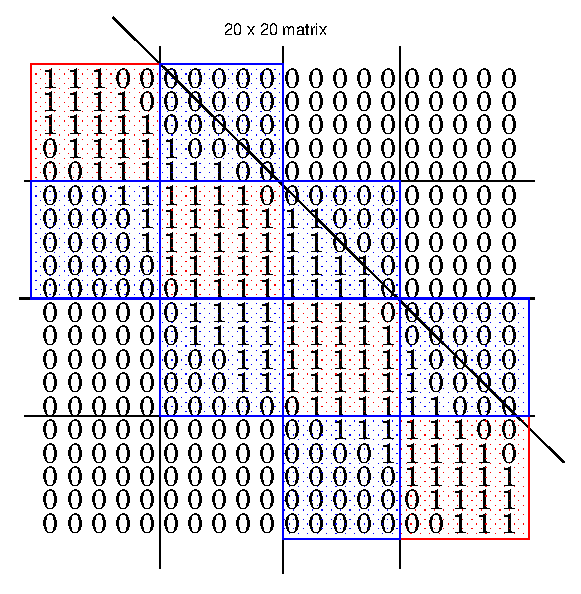
\includegraphics[scale=1.0]{deciexamp.eps}
%\begin{minipage}{4in}
%\epsfxsize=4in \epsfysize=4in \centerline{\epsfbox{deciexamp.eps}}
%\end{minipage}
\end{center}
\caption{Form of the Dyson equation, and the principal layer concept
each 0 and 1 correspond to an LMMAX x LMMAX matrix (i.e. LMMAX=16 for 
$l_{\rm max} = 3$). 
The line demonstrates a simple way to find the size of the 
principal layers which is 5 in this example}
\label{fig1}
\end{figure}    



\subsection{Current calculation}
Parameters for Current formula calculation
 IEGFOUT=14
 ZCURR1=1.5d0         ZCURR2= 5.0d0       RMTCURR=0.25d0

For the current formula only the Energy IEGFOUT is used
the current is calculated between planes z=ZCURR1 and z= ZCURR2
Running Option CONDUCT should be used.
The appropriate files for further calculation are written out:
greenfun, fort.66 holds the wavefunctions. You should run it in 
one iteration mode! The IGF parameter should also be set to one
IGREENFUN=1. The output is used by the current programs...  


\section{Examples}

\subsection{Fe Bulk}

Example for bcc Fe! In the following example only numbered
lines are really necessary.
All parameters are explained in the text a few comments are added here.  

{\tt {\small
 
\begin{tabbing}
% dont show this
xxxx\=xxxxxxxxxxxx\=xxxxxxxxxxxxx\=xxxxxxxxxxxx\=xxxxxxxxxxx\=xxxxxxxxxx\kill
***** Input file for TB-KKR code *****         \\
      ***Running options***                    \\
1 \>RUNOPT                                     \\
2 \>full inv                                   \\
  \>+-------+-------+-------+-------+-------+  \\ 
  \>     ***test options*** (2 lines)          \\
3 \>TESTOPT                                    \\
4 \>ie                                         \\
5 \> ....    .....                             \\
  \>+-------+-------+-------+-------+-------+  \\
6 \>LMAX=3   \> NSPIN=2   \>NATYP= 1 \> KMT=3  \\  
  \>-------------------------------------------- \\
  \>** Description of lattice**                  \\
7 \>ALATBASIS= \>5.220 \>    1.0  \>    1.0   \>     lattice constants \\
8 \>BASISCALE= \>1.0   \>    1.0  \>    1.0   \>     scaling factor    \\
9 \>LATTICE=1                 \\
10\>BRAVAIS                   \\
11\>     \> -0.500000  \>  0.500000 \>  0.500000  \\
12\>     \>  0.500000  \> -0.500000 \>  0.500000  \\
13\>     \>  0.500000  \>  0.500000 \> -0.500000  \\
  \>---------------------------------------------------------------------- \\
14\>NAEZ= 1  \> NEMB=0   \>NEMBZ=0  \>KAOEZ=0 \\
15\>CARTESIAN= f     \\
16\>RBASIS \\
17\>      0.00000000 \>  0.00000000 \> 0.00000000  \>    1 \\
18\>SCALING= \> 1.0    \>     1.0  \>       1.0\\
\>---------------------------------------------------------------------- \\
19\>INTERFACE= F \\
20\> NRIGHTHO=  \>10  \>  NLBASIS=  1 \\
21\> NLEFTHOS=  \>10  \>  NRBASIS=  1 \\
22\> LEFTBASIS   \> x    \>     y   \>      z  \>   refpot \\
23\> \>        0.50000000 \>  0.50000000 \> -0.50000  \>   1 \\
24\> RIGHBASIS \\
25\>     \>     0.00000000 \>  0.00000000  \> 8.00000 \>    1 \\
\>--------------------------------------- \\
26\>ZPERIODL=\> 0.50000000 \> 0.50000000 \> -0.50000000 \\
27\>ZPERIODR=\> 0.50000000 \> 0.50000000 \>  0.50000000 \\
\>---------------------------------------------------------------------- \\
\>Parameters for the clusters    (if same spherical cluster else cylindrical) 
\\
28\> RCLUSTZ=\>2.00d0  \>     RCLUSTXY=\>2.00d0 \\
\>---------------------------------------------------------------------- \\
\end{tabbing}
\begin{tabbing}
% dont show this
xxxx\=xxxxxx\=xxxxxx\=xxxxxxxxx\=xxxxx\=xxxxxxxxxx\=xxxxx\=xxxxxxx\=xxxxxxx\=xxxxxxx\=xxxxxxx\kill
29\>ATOMINFO \\
30\>Z   \> LMXC\> KFG     \> CLS \> REFPOT \> NTC  \>  FAC  \> IRNS \> RMT  \> 
WEIGHT \\
31\>26.0 \> 1  \> 3 3 0 0 \>  1  \>  1     \>  1   \>  1.00 \> 208  \>  2.00\> 
1.00 \\ 
\end{tabbing}
\begin{tabbing}
% dont show this
xxxx\=xxxxxxxxxxxxxxxxx\=xxxxxxxxxxxxxxxxxx\=xxxxxxxxxxxxxx\=xxxxxxxxxx\=xxxxxxxx\=xxxxxxxx\=xxxxxxx\kill
\>---------------------------------------------------------------------- \\
32\>EMIN  \>     EMAX    \>   TEMPR   \>   NPOL \>  NPT1 \>  NPT2 \>    NPT3 \\
33\>-0.30 \>    .8461000 \>  500.00d0 \>   5    \>   3   \>   20  \>     3   \\
\> Chose the emin carefully, look at the positions of the core states \\
\> in the potential cards and the voronoi output! \\
\>---------------------------------------------------------------------- \\
34\>  IRNUMX= 10 \>ITCCOR= 40 \>   IPRCOR= 1   \> IFILE= 13   \>     IPE= 0 \\
35\>     KWS= 2    \>KSHAPE= 2  \>      IRM= 484 \>     INS= 1  \>   ICST= 2 \\
\> For asa change KSHAPE=0, IRM=353 (usual), INS=0 \\
36\>  INSREF= 0    \>   KCOR= 2 \>     KVREL= 0  \>   KEXCOR= 2 \\
37\> KHYPERF= 0    \>KHFIELD= 0 \>      KEFG= 0  \\
38\>     KTE= 0    \>   KPRE= 0  \>    KVMAD= 0  \> KSCOEF= 0 \\
39\> IPOTOUT= 1    \>IGREENFUN= 0  \>      ICC= 0 \>  ISHIFT= 0 \\
40\>  HFIELD= 0.0  \> VCONST= 0.0d0 \>KFORCE= 0   \\
41\> BZDIVIDE= \> 30  \>   30   \>  30\\
\>---------------------------------------------------------------------- \\
\end{tabbing}
\begin{tabbing}
% dont show this
xxxx\=xxxxxxxxxxx\=xxxxxxxxxx\=xxxxxxxxxxxxxx\=xxxxxxxxxx\=xxxxxxxxxx\=xxxxxxxxxxx\=xxxxxxxxx\kill
42\>NSTEPS  \>   IMIX  \>  STRMIX  \>     FCM  \>     QBOUND \>   BRYMIX  \>   
 ITDBRY \\
43\> 15     \>    5    \>    0.01 \>     20.0 \>     1.D-6 \>     0.0050 \>    
  10  \\
\> The parameters below are obsolete but are read in for backward 
compatibility \\
\>---------------------------------------------------------------------- \\
\>LINIPOL= f      LRHOSYM=f    LCOMPLEX= f \\
\>Center of inversion :      NZ=4     LCENTER= t \\
\> LOGINV= f       INIPOL= 0     IXIPOL=  0  \\
\>CENTROFIN=   0.0      0.0      0.0  \\
\>---------------------------------------------------------------------- \\
\>MMIN= 1   MMAX=6                      mmin mmax (bands) \\
\>SRINOUT=   0   0   0  00              sinn(0/1)sout(0/23)rin(0/1)rout(0/17) 
\\
\> end of obsolete parameters \\
\>---------------------------------------------------------------------- \\
44\>FILES \\
45\>4Ryshift    \>          \>\>\>                        I12 \\
46\>potential   \>          \>\>\>                        I13 \\
47\>madelung       \>       \>\>\>                        I40 \\
48\>shape00        \>       \>\>\>                        I19 \\
49\>scoef          \>       \>\>\>                        I25 \\
\>----------------------------------------|40--------------------------- \\
\> Potential names are 40 characters long, if the program stops    \\
\> trying to open an unneaded file i.e. scoef or shape althought you are in 
asa mode\\
\> then just create empty files with these names! \\
50\>DECIFILES \\
51\>fedeci.fp1 \\
52\>fedeci.fp2 \\
\>---------------------------------------------------------------------- \\
\>Parameters for ewald sums \\
53\>RMAX=\>5.0d0  \>   GMAX=\>50.0d0 \>    (fcc 7  65) \\ 
\>--------------------End of inputcard---------------------------------- \\
\end{tabbing}
}} % end tt small

Now we will present a few more examples. Since only the lattice is needed
to change and all the rest of the parameters remain the same we will give
examples for the fcc, bcc, and some decimation
example with decimating one and 2 atoms. Only the parameters that are relevant
are given. Each line has a numbering which is used only in 
the manual for reference. 

% ----------------------------------------------------------------

\subsection{FCC Bulk Lattice}
{ \tt {\small
\begin{tabbing}
% dont show this
xxxx\=xxxxxxxxxxxx\=xxxxxxxxxxxxx\=xxxxxxxxxxxx\=xxxxxxxxxxx\=xxxxxxxxxx\kill
  \>** Description of lattice**                  \\
7 \>ALATBASIS= \>6.76  \>    1.0  \>    1.0   \>     lattice constants \\
8 \>BASISCALE= \>1.0   \>    1.0  \>    1.0   \>     scaling factor    \\
10\>BRAVAIS                   \\
11\>     \>  0.500000  \>  0.500000 \>  0.000000  \\
12\>     \>  0.500000  \>  0.000000 \>  0.500000  \\
13\>     \>  0.000000  \>  0.500000 \>  0.500000  \\
  \>---------------------------------------------------------------------- \\
14\>NAEZ= 1  \> NEMB=0   \>NEMBZ=0  \>KAOEZ=0 \\
15\>CARTESIAN= f     \\
16\>RBASIS \\
17\>         0.00000000 \>  0.00000000 \> 0.00000000  \>    1 \\
18\>SCALING= \> 1.0    \>     1.0  \>       1.0\\
\>---------------------------------------------------------------------- \\
19\>INTERFACE= F \\
\end{tabbing}
% -------------------------------------------------------------
}} % tt small
\subsection{FCC bulk in 001 surface geometry}
{\tt{\small
\begin{tabbing}
% dont show this
xxxx\=xxxxxxxxxxxx\=xxxxxxxxxxxxx\=xxxxxxxxxxxx\=xxxxxxxxxxx\=xxxxxxxxxx\kill
  \>** Description of lattice**                  \\
7 \>ALATBASIS= \>6.76  \>    1.0  \>    1.0   \>     lattice constants \\
8 \>BASISCALE= \>1.0   \>    1.0  \>    1.0   \>     scaling factor    \\
10\>BRAVAIS                   \\
11\>     \>  0.70710678  \>  0.000000   \>  0.000000  \\
12\>     \>  0.000000    \>  0.70710678 \>  0.000000  \\
13\>     \>  0.35355339  \>  0.35355339 \>  0.500000  \\
  \>---------------------------------------------------------------------- \\
14\>NAEZ= 1  \> NEMB=0   \>NEMBZ=0  \>KAOEZ=0 \\
15\>CARTESIAN= f     \\
16\>RBASIS \\
17\>         0.00000000 \>  0.00000000 \> 0.00000000  \>    1 \\
18\>SCALING= \> 1.0    \>     1.0  \>       1.0\\
\>---------------------------------------------------------------------- \\
19\>INTERFACE= F \\
\end{tabbing}
}}% tt small
\subsection{FCC 001 surface with 8 atom slab}
{\tt {\small
\begin{tabbing}
% dont show this
xxxx\=xxxxxxxxxxxx\=xxxxxxxxxxxxx\=xxxxxxxxxxxx\=xxxxxxxxxxx\=xxxxxxxxxx\kill
6 \>LMAX=3   \> NSPIN=2   \>NATYP= 8 \> KMT=3  \\  
  \>** Description of lattice**                  \\
7 \>ALATBASIS= \>6.76  \>    1.0  \>    1.0   \>     lattice constants \\
8 \>BASISCALE= \>1.0   \>    1.0  \>    1.0   \>     scaling factor    \\
10\>BRAVAIS                   \\
11\>     \>  0.70710678  \>  0.000000   \>  0.000000  \\
12\>     \>  0.000000    \>  0.70710678 \>  0.000000  \\
13\>     \>  0.000000    \>  0.0000000 \>   0.000000  \\
  \>---------------------------------------------------------------------- \\
14\>NAEZ= 8  \> NEMB=0   \>NEMBZ=0  \>KAOEZ=0 \\
15\>CARTESIAN= f     \\
16\>RBASIS \\
17\>         0.00000000 \>  0.00000000 \> 0.00000000   \\
  \>       0.50000000   \>0.50000000 \> 0.50000000     \\
  \>       0.00000000   \> 0.00000000  \> 1.00000000   \\
  \>       0.50000000   \> 0.50000000  \> 1.50000000    \\ 
  \>       0.00000000   \> 0.00000000  \> 2.00000000    \\
  \>       0.50000000   \> 0.50000000  \> 2.50000000    \\ 
  \>       0.00000000   \> 0.00000000  \> 3.00000000    \\
  \>       0.50000000   \> 0.50000000  \> 3.50000000    \\
18\>SCALING= \> 1.0    \>     1.0  \>       1.0\\
\>---------------------------------------------------------------------- \\
19\>INTERFACE= T \\
20\> NRIGHTHO=  \>10  \>  NLBASIS=  1 \\
21\> NLEFTHOS=  \>10  \>  NRBASIS=  1 \\
22\> LEFTBASIS   \> x    \>     y   \>      z  \>   refpot \\
23\> \>        0.50000000 \>  0.50000000 \> -0.50000  \>   1 \\
24\> RIGHBASIS \\
25\>     \>     0.00000000 \>  0.00000000  \> 4.00000 \>    1 \\
\>--------------------------------------- \\
26\>ZPERIODL=\> 0.50000000 \> 0.50000000 \> -0.50000000 \\
27\>ZPERIODR=\> 0.50000000 \> 0.50000000 \>  0.50000000 \\
\end{tabbing}
% ------------------------------------------------------------- 
}} % tt small
\subsection{SUPERCELL}
You can very easily 
go from a slab (look previous example) or a decimated interface to a repeated 
supercell calculation. 
In the above 8 atom slab example you make a supercell  
 by just using in line 19 INTERFACE=F and changing
line 13 to 0.0  0.0   4.0 . Then your system is periodically repeated.
 A different fast  algorithm will be used to invert 
the Dyson in this case since the matrix is not a simple band diagonal matrix 
any more.     
Alternatively you could use option 'sparse'.
 The size of the
principal layer is found in a similar way as demonstrated earlier in this 
manual.
If you are not sure that the 
fast inversion algorithm will work in your case you can always use "full inv" 
to make
Full inversion. Note here that the LATTICE=1 (line 9 on Fe bulk example) 
should 
also be changed to something like LATTICE=2 (or any other number)
or else you would be using the 2D k-points in your
3D supercell calculation. Alternatively you can erase all k-points files
in the mesh directory to be sure that correct k-points are created.

\subsection{Fe/ZnSe/Fe interface with 2 different Fe atoms in plane
using decimation}

This is a rather complicated example which has 2 atoms in plane, 
and it is doing 
decimation on both sides while empty spheres 
are included for the semiconductor.
This is to demonstrate how you set up the lattice in case of decimation and
if you need to decimate more than one atom. Try to visualize the lattice.
{\tt {\small
\begin{tabbing}
% dont show this
xxxxxx\=xxxxxxxxxxxx\=xxxxxxxxxxxxx\=xxxxxxxxxxxx\=xxxxxxxxxxx\=xxxxxxxxxx\kill
6 \>LMAX=3   \> NSPIN=2   \>NATYP= 16 \> KMT=3  \\  
  \>** Description of lattice**                  \\
7 \>ALATBASIS= \>10.41  \>    1.0  \>    1.0   \>     lattice constants \\
8 \>BASISCALE= \>1.0   \>    1.0  \>    1.0   \>     scaling factor    \\
10\>BRAVAIS                   \\
11\>     \>  0.500000    \>  0.500000   \>  0.000000  \\
12\>     \> -0.500000    \>  0.5000000 \>   0.000000  \\
13\>     \>  0.000000    \>  0.0000000 \>   0.000000  \\
\>---------------------------------------------------------------------- \\
14\>NAEZ= 16  \> NEMB=0   \>NEMBZ=0  \>KAOEZ=0 \\
15\>CARTESIAN= f     \\
16\>RBASIS \\
17a  \>       0.00000000  \> 0.00000000 \> 0.00000000    \\
17b  \>       0.50000000  \> 0.50000000 \> 0.00000000  \\
17c  \>       0.50000000  \> 0.00000000 \> 0.25000000\\
17d  \>       0.00000000  \> 0.50000000 \> 0.25000000\\
17e  \>       0.00000000  \> 0.00000000 \> 0.50000000\\
17f  \>       0.50000000  \> 0.50000000 \> 0.50000000\\
17g  \>       0.50000000  \> 0.00000000 \> 0.75000000\\
17h  \>       0.00000000  \> 0.50000000 \> 0.75000000\\
17j  \>       0.00000000  \> 0.00000000 \> 1.00000000\\
17k  \>       0.50000000  \> 0.50000000 \> 1.00000000\\
17l  \>       0.50000000  \> 0.00000000 \> 1.25000000\\
17m  \>       0.00000000  \> 0.50000000 \> 1.25000000\\
17n  \>       0.00000000  \> 0.00000000 \> 1.50000000\\
17o  \>       0.50000000  \> 0.50000000 \> 1.50000000\\
17p  \>       0.50000000  \> 0.00000000 \> 1.75000000\\
17q  \>       0.00000000  \> 0.50000000 \> 1.75000000\\
18\>SCALING= \> 1.0    \>     1.0  \>       1.0\\
\>--------------------------------------------------------------------- \\
19\>INTERFACE= T \\
20\> NRIGHTHO=  \>10  \>  NLBASIS=  2 \\
21\> NLEFTHOS=  \>10  \>  NRBASIS=  2 \\
22\> LEFTBASIS   \> x    \>     y   \>      z  \>   refpot \\
23\> \>        0.00000000 \>  0.50000000 \> -0.250000  \>   1 \\
23a  \> \>        0.50000000 \>  0.00000000 \> -0.250000  \>   2 \\ 
24\> RIGHBASIS \\
25\>     \>     0.00000000 \>  0.00000000  \> 2.00000 \>    1 \\
25a \>     \>     0.50000000 \>  0.5000000   \> 2.00000 \>    2 \\
\>---------------------------------------------------------------------- \\
26\>ZPERIODL=\> -0.50000000 \> 0.00000000 \> -0.250000000 \\
27\>ZPERIODR=\> 0.50000000 \> 0.00000000 \>  0.250000000 \\

\end{tabbing}
}} % tt small
We also give the atomic information for this case notice that the 
parent lattice is bcc, this means that the tb-clusters are bcc!
{\tt {\small
\begin{tabbing}
% dont show this
xxxxxx\=xxxxxx\=xxxxxx\=xxxxxxxxx\=xxxxx\=xxxxxxxxxx\=xxxxx\=xxxxxxx\=xxxxxxx\=xxxxxxx\=xxxxxxx\kill
29\>ATOMINFO \\
30\>Z   \> LMXC\> KFG     \> CLS \> REFPOT \> NTC  \>  FAC  \> IRNS \> RMT  \> 
WEIGHT \\
31a\>26.0 \> 1  \> 3 3 0 0 \>  1  \>  1     \>  1   \>  1.00 \> 208  \>  
2.00\> 1.00 \\
31b\>26.0 \> 1  \> 3 3 0 0 \>  1  \>  1     \>  1   \>  1.00 \> 208  \>  
2.00\> 1.00 \\
31c\>26.0 \> 1  \> 3 3 0 0 \>  1  \>  1     \>  1   \>  1.00 \> 208  \>  
2.00\> 1.00 \\
31d\>26.0 \> 1  \> 3 3 0 0 \>  1  \>  1     \>  1   \>  1.00 \> 208  \>  
2.00\> 1.00 \\
31e\>30.0 \> 1  \> 3 3 0 0 \>  1  \>  1     \>  1   \>  1.00 \> 208  \>  
2.00\> 1.00 \\
31f\> 0.0 \> 0  \> 0 0 0 0 \>  1  \>  1     \>  1   \>  1.00 \> 208  \>  
2.00\> 1.00 \\
31g\>34.0 \> 2  \> 3 3 3 0 \>  1  \>  1     \>  1   \>  1.00 \> 208  \>  
2.00\> 1.00 \\
31h\> 0.0 \> 0  \> 0 0 0 0 \>  1  \>  1     \>  1   \>  1.00 \> 208  \>   
2.00\> 1.00 \\
31j\> 0.0 \> 0  \> 0 0 0 0 \>  1  \>  1     \>  1   \>  1.00 \> 208  \>  
2.00\> 1.00 \\
31k\>30.0 \> 1  \> 3 3 0 0 \>  1  \>  1     \>  1   \>  1.00 \> 208  \>  
2.00\> 1.00 \\
31l\>0.0 \> 0  \> 0 0 0 0 \>  1  \>  1     \>  1   \>  1.00 \> 208  \>   
2.00\> 1.00 \\
31m\>34.0 \> 2  \> 3 3 3 0 \>  1  \>  1     \>  1   \>  1.00 \> 208  \>  
2.00\> 1.00 \\
31n\>30.0 \> 1  \> 3 3 0 0 \>  1  \>  1     \>  1   \>  1.00 \> 208  \>  
2.00\> 1.00 \\
31o\>0.0 \> 0  \> 0 0 0 0 \>  1  \>  1     \>  1   \>  1.00 \> 208  \>   
2.00\> 1.00 \\
31p\>26.0 \> 1  \> 3 3 0 0 \>  1  \>  1     \>  1   \>  1.00 \> 208  \>  
2.00\> 1.00 \\
31q\>26.0 \> 1  \> 3 3 0 0 \>  1  \>  1     \>  1   \>  1.00 \> 208  \>  
2.00\> 1.00 \\
\end{tabbing}
% ------------------------------------------------------------- 
}} % tt small

The bulk calculation to produce the decimation files for the above should have 
a
lattice 
{\tt {\small
\begin{tabbing}
% dont show this
xxxx\=xxxxxxxxxxxx\=xxxxxxxxxxxxx\=xxxxxxxxxxxx\=xxxxxxxxxxx\=xxxxxxxxxx\kill
10\>BRAVAIS                   \\
11\>     \>  1.00000    \>  1.000000   \>  0.000000  \\
12\>     \> -1.000000    \>  1.0000000 \>   0.000000  \\
13\>     \>  0.500000    \>  0.5000000 \>   0.500000  \\
15\>CARTESIAN= f     \\
16\>RBASIS \\
17a  \>       0.00000000  \> 0.00000000 \> 0.00000000    \\
17b  \>       0.50000000  \> 0.50000000 \> 0.00000000  \\
\end{tabbing}
}} % tt small
Finally one small remark about supercell calculations. 
In the above Fe/ZnSe/Fe example you make a supercell  
 by just using in line 19 INTERFACE=F and changing
line 13 to 0.0  0.0   2.0 . Then your system is periodically repeated. 
Of course you should not use the DECIMATE running options.



%----------------------------------------------------------
The BCC bravais vectors are:
{\tt {\small
\begin{tabbing}
% dont show this
xxxx\=xxxxxxxxxxxx\=xxxxxxxxxxxxx\=xxxxxxxxxxxx\=xxxxxxxxxxx\=xxxxxxxxxx\kill
10\>BRAVAIS                   \\
11\>     \> -0.500000  \>  0.500000 \>  0.500000  \\
12\>     \>  0.500000  \> -0.500000 \>  0.500000  \\
13\>     \>  0.500000  \>  0.500000 \> -0.500000  \\
  \>---------------------------------------------------------------------- \\
\end{tabbing}
}}
%FCC
%FCC 001
%FCC 111
%FCC 110
%BCC 001
%BCC 111
%BCC 110
%Zink blende with 2 empty spheres
%NaCl
%more lattice structures: 


\section{TEST options}
Like 
in the case of the RUNNING OPTIONS there exist also the TEST OPTIONS that are
also 8 characters length and that are used to make several tests in the code 
when
active. This provides an efficient way to add also new tests by just using an 
if statement.
We just provide the names of the most important ones and someone 
should refer to the code itself to find out the functionality of each one:
\medskip

\noindent
{\tt {\small
        clusters,
        clscoor,
        shells,
        spec cls,
        ND,  
        deltall,
        BZKP, 
        NoSymGnn,
        flow,
        INGSP,
        ingsp, \\
        \mbox{fix sym},
        eigen0,
        spec RMT,
        tmat,
        HARDCORE,
        spec RMT,
        pznorm,
        setTzero,
        tmatll1,
        www, \\
        cc, 
        gllke,
        e(k),
        k-net,
        fix E2,
        EV, 
        nbasis,
        fix NE,
        e-scan1,
        e-scan,
        simpl E,
        ip-scan, \\
        sub ef, 
        larg\_acc,
        at ef,
        no ef-de,
        no ef+de,
        no ef,
        UP,
        DOWN,
        NFE,
        eigiso,
        lay ind, \\
        C(L),
        NFE,
        noqshift,
        qs\_out,
        csq(L),
        phase(i),
        larg\_acc,
        NoMadel,
        electro,
        N1 N2, 
        GFREE,
        REFPOT,
        WAIT,
        RROT,
        k-net,
        crt mesh,
        k-mesh,
        nikos,
        RMESH,
        EXARG,
        TINVLL,
        latshell, \\
        c/a,
        opt mix, 
        pot head,
        IE=1,
        e-net,
        fix mesh,
        DOS,
        EV,
        ONE-E,
        ie,
        grefll,
        spec RMT, \\
        trefll,
        Tphase,
        LLOYD,
        gmatll,
        sub ef,
        rhons,
        alt mix,
        spec mix,
        VBC,
        testpzsq,
        GMAT, \\
        IMAD,
        RR,
        madelsum,
        GLL0,
        STRING,
        CONT,
        cmom.   \\ \\
}} % tt small
%--------------------------------------------
\section{Inputcard}

The inputcard contains all the information needed on the system and the 
calculation.
In this paragraph we analyze all the input parameters and the construction
of this file. 

 A few remarks on the format of this file: 
Comments can be included and are ignored from the program, only 
data after the codewords are read in. You can place the codewords
anywhere in the inputcard. Codewords have to be in uppercase so you can
keep comments in lowercase. If a codeword is directly followed by an equal 
sign (=)
the number(s) in the same line following the codeword will be read in. If no 
equal sign is present the value which is exactly below the 
codeword will be read in.
This is explained more in subroutine "ioinput.f".    

The first line contains the so called 
running options (lines 1-2) in the example. There is a list of options mostly
used to take out a specific quantity or impose a condition to
the calculation. The program for the RUNNING OPTIONS always reads 
everything in strings of 8 characters, so be careful when you have more
than one option. The most important running options are\\

\begin{tabular}{ll}
       {COMPLEX}   &  Complex band structure plots (1 iteration)\\
       {BAND-STR}  &  Band structure plots (1 iteration)      \\
       {symG(k)}   &  \\
        T\_hcore&\\
        rigid-ef    & The Ef is fixed during iterations \\
        full inv    & doesn't use O(N) algorithm for matrix inversion\\
                    & this is usually used for bulk calculations \\
                    & but it depends on the form of the Dyson equation\\
                    & for long supercells you can use the O(N) algorithm\\
        sparse      & Sparse matrix inversion \\
                    & (not possible with decimation yet \\
        deci-out    & write out the t-matrix in 'decifile'\\
        DECIMATE    & use decimation technique\\
        DECIMATEONEBULK &  Speed up decimation, step information used for\\ 
        &              the left bulk is just copied to the right one. \\
        cut Four&\\
        DOS-EF&\\
        DOS REF&\\
        QDOS         & q-dos calculation (1 iteration )      \\
        CURRENT      & current calculation (1 iteration) \\
        CONDUCT & \\
       GENPOT    & generates the file fort.3 which contains the potential \\
           & in a special format. Refer to the part on the \\ & VORONOI for 
more details.

\end{tabular}

%-----------------------------



%-------------------------------------------------------------------------------\\
\begin{tabbing}
xxxxxxxxxxxxxx\=xxxxxxxxxxxxxxxxxxxxxxxxxxxxxxxxxxxxxxxxxxxxxxxxxxx\kill 
\underline{LMAX} : \> value of l-cut-off for wavefunctions, a value of 2*lmax 
is used for the \\
  \> charge moments. Normally 2 is good only for the spin moments, \\
  \>3 for the energies and someone should use at least 4 for the forces\\
\underline{NSPIN} :\> number of spins (2: spin-polarized, 1: paramagnetic)\\
\underline{NATYP} :\> number of inequivalent sites in the system 
               (must be the same as NAEZ) \\
\underline{KMT=3} \> (not used anymore)\\ \\


%-------------------------------------------------------------------------------\\
\ \\
{\bf Description of the lattice }\\
\ \\
\underline{ALATBASIS} :\> lattice parameters in atomic units (a, b/a, c/a)\\
\underline{BASISCALE} :\> the atomic coordinates are divided by the BASISCALE 
numbers\\
\underline{LATTICE}  :\> Gives the name in the k-points file, it can be any 
integer positive number \\
\underline{BRAVAIS}  :\> Bravais vectors in terms of ALATBASIS, Each line 
corresponds to one vector. \\
\>If someone does surfaces, he has just a two dimensional periodicity, the 
third \\ 
\>Bravais lattice should be (0.0, 0.0, 0.0) and the $z$ component of the first 
two  \\
\>Bravais vectors should be also 0.0  \\

%-------------------------------------------------------------------------------\\
\underline{NAEZ} :\> same as NATYP\\
\underline{NEMB} :\>   not used\\
\underline{NEMBZ} :\>  not used  \\
\underline{KAOEZ} :\>  not used \\
\underline{CARTESIAN} : \> f or t (false or true). \\ 
        \phantom{CARTESIAN=} \>          false: if the atomic coordinates and 
\\
                   \>  the vectors are expressed in units of the Bravais 
vectors (Wyckoff coordinates). \\
  \phantom{CARTESIAN=}\>       true: if the atomic coordinates are Cartesian 
coordinates \\
                      \>  independent of the Bravais vectors.\\
\ \\
\underline{RBASIS}: \> coordinates of the Basis atoms, in 2d geometry these 
are the\\
               \> coordinates of the different atoms which have the same \\
               \> 2d geometry (i.e. belong in different planes, or in 
different \\
               \> sub lattices in the same plane if we have more atoms in the 
same plane) \\
\ \\ 
             \>   Important for the scaling is that in case of 2d geometry \\  
             \>   i.e. INTERFACE=.true. the z-component of the BRAVAIS    \\
             \>   is always zero. This means that in this case the z-component 
 \\
             \>   of RBASIS is always in Cartesian coordinates. \\
%-------------------------------------------------------------------------------\\

\underline{SCALING} : \> scaling (usually not used) Scaling done with 
BASISCALE\\

%-------------------------------------------------------------------------------\\
\underline{INTERFACE:} \> true (T) or false (F). \\
\phantom{INTERFACE:}  \> T :  2 - D Geometry \\
\phantom{INTERFACE:}  \> F :  3 - D Geometry (Periodically repeated)\\
\end{tabbing}
%-------------------------------------------------------------------------------\\
   The following variables are used in the case of 2D geometry. In the case of
slab calculation the information is used to produce the TB-clusters which for 
the
boundary atoms extend outside the
slab region. In the case of semi-infinite geometry (decimation) they have the
extra role of defining the lattice outside our active region and this 
information is used to calculate the electrostatic potential of the 
semi-infinite system which converges fast since you have to add charge neutral 
blocks of layers. Look later in the manual
 for a more detailed description of the role of these parameters.\\

\begin{tabbing}
xxxxxxxxxxxxxxxx\=xxxxxxxxxxxxxxxxxxxxxxxxxxxxxxxxxxxxxxxxxxxxxxxxxxxxx\kill 

\underline{NRIGHTHO} : \>number of layers taken into account right of the 
system. \\
\underline{NLBASIS} : \> number of basis vectors to construct the right part 
of 
         the system\\
\underline{NLEFTHOS} : \> same as NRIGHTHO, but left of the system\\
\underline{NRBASIS} :\>  same as NLBASIS for the right part.\\
\underline{LEFTBASIS} \> (X, Y, Z, REFPOT) vectors to construct the next layer 
on the 
          left side. \\
       \>   Gives the coordinate of the inequivalent sites on the layer 
          relative to the origin. \\
\underline{RIGHBASIS} :\> (X, Y, Z, REFPOT) same but on the right side. \\
\underline{ZPERIODL} :\> vector  to construct the next layer on the left side. 
\\ 
              \>    Gives the coordinate of the inequivalent sites on the 
layer \\
              \>    relative to the origin. \\
\underline{ZPERIODR} :\>  same on the right side\\


%-------------------------------------------------------------------------------\\
\> \bf{Parameters for the TB-structure constants cluster}\\

\underline{RCLUSTZ},  \\
\underline{RCLUSTXY} : \> radius (scaled with alat) determining the size of \\ 
               \> the TB-cluster (along z axis, and x y axes)  \\
               \>           (if equal, spherical cluster else cylindrical 
cluster) \\
 \> The size of the cluster is written out, and it also affects \\
 \> the size of the principal layer \\ 
\underline{ATOMINFO} : \> description of core states and atom depending 
properties\\
           \> The next line is comment line and then NATYP lines are needed \\
\underline{Z} : \> nuclear charge\\
\underline{LMXC} :\> lmax core,  \\
\phantom{LMXC  } \> argon core:  lmxc = 1 \\
\phantom{LMXC  } \> krypton:     lmxc = 2\\
\phantom{LMXC  } \> xenon:       lmxc = 3\\
\underline{KFG} : \>    configuration of core electrons:  \\
\phantom{KFG= } \> argon core:   3 3 0 0=3s,3p (3d series)\\
\phantom{KFG= } \> krypton core: 4 4 3 0=4s,4p,3d (4d series)\\
\phantom{KFG= } \>  xenon core+4f:   5 5 4 4=5s,5p,4d,4f (5d series)\\
\underline{CLS:}  \>  type of cluster, used in case of structures with more
                than one type of TB-cluster \\
                \> This information is not used by the voronoi program but is 
needed in the kkr. \\
                \> The voronoi provides this info in it's output and should be 
taken from there.\\
\underline{REFPOT} :\>      used to set reference potentials of different 
heights or\\
\> different MT radii for each basis atom. More potentials are needed in the 
\\
\> 4Ryshift file in this case usually set to 1 \\   
\underline{NTC} :   \>      indexes different shape functions in case of atoms 
with \\
     \> different geometric environment this information is provided by 
voronoi also. \\
 \> Look at the part on how to get the initial potential and the shape 
functions \\
 \> for more details.\\
\underline{FAC}: \>         not used set to 1.00\\
\underline{IRNS} : \>        number of radial points where the potential is 
non 
                     spherical, \\
               \> but counted from the maximum radius in. Usually set to 208
               or 278
               \\
\underline{RMT}: \>  Muffin-tin sphere in the case of FP calculations. This is 
important and \\
    \> sets up the so-called muffin-tinization of the potential, used only by 
voronoi\\
\underline{WEIGHT}: \> weight of each atom when the voronoi polyhedra are 
constructed. \\
\>For both RMT and WEIGHT look at the part on how to get the initial potential 
\\
\>and the shape functions for more details.\\ 

\\
%------------------------------------------------------------------------------- 
\\
\bf{Energy contour} \\
\underline{EMIN}: \> lower energy of contour \\
\underline{EMAX}: \>  Maximum energy (in self consistent calculations \\
           \>   The Fermi level is read from the potential card). Attention 
the energies \\
\> for the integration should be such that they do not include any core states 
and \\
\> do not leave out any valence states. You can see the energetic position \\
\> of the core states in the potential cards. \\
\>               In case of DOS calculation EMAX is used.\\
\ \\
\>  For the energy integration a rectangular contour with npt2 points parallel 
\\
\>  to the real axis is used. \\
\ \\
\underline{TK}: \> temperature in Kelvin (determines the distance from the real
             axis) \\
\> Look at Phys. Rev. B 52, 11502 (1995) \\
\ \\
\underline{NPOL}: \> number of Matsubara poles for complex integration with 
temperature \\
             \>   if NPOL=0, the DOS if written out with NPT2 energy points. \\
\underline{NPT1,2,3}: \>number of energies points for complex integration\\
\phantom{NPT1,2,3=}  \>                npt2 points parallel to real axis,\\
\phantom{NPT1,2,3=}  \>                 npt1 points used to go up from the 
real axis\\
\phantom{NPT1,2,3=}  \>                 npt3 points used to go down to the 
real axis\\
%-------------------------------------------------------------------------------\\

\underline{IRNUMX}: \> obsolete set to 10!  \\
\underline{ITCCOR}: \> Iterations for determining the core state energy, 40 is 
enough.\\
\underline{IRPCORE}: \> Print information about the core states\\
\underline{IFILE}: \>  \\
\underline{IPE}: \>  not used ???\\
\underline{KWS}:\> 1 for  MT, 2 for ASA\\
\underline{KSHAPE}: \> shape function for exact treatment of the potential \\ 
   \> 0=ASA, \\ 
   \> 1=the potential is replaced by a constant at the RMT (this is useful 
sometimes) \\
   \> 2=correct Full Potential \\
\underline{IRM}: \> number of points on the radial space mesh in the MT 
sphere.\\
\> Normally we use 353 points for the ASA calculations and 484 for the FP 
Calculations \\
\underline{INS}: \> 0 for ASA, 1 for FP \\
\underline{ICST}: \> number of iterations in the Born scheme (for FP 
calculation).\\
\> The Born scheme is used to derive the $R_{LL'}$  wavefunctions needed \\ 
\> for the FP calculation from the $R_{L}$ wavefunctions (solutions of the \\
\> radial Schr\"odinger equation) using the Lippman-Schwinger. Normally 2-3 \\
\> iterations are enough. The criterion is converged total energies and/or 
forces\\
\underline{INSREF}: \> 0 MT screening, 1 FP screening (set it to 0 )\\
\underline{KCOR:} \> core relaxation: \\
\phantom{KCOR=}\> KCOR=0 no core relaxation (frozen core calculation)\\
\phantom{KCOR=}\>  KCOR=1 SRA core relaxation \\
\phantom{KCOR=}\> KCOR=2 non-SRA core relaxation \\
\underline{KVREL}: \>Scalar relativistic calculation\\
\phantom{KVREL=} \> KVREL=0 non relativist calculation  \\
\phantom{KVREL=} \>  KVREL=1 SRA calculation\\
\underline{KEXCOR}:\> exchange-correlation (0=von Barth Hedin, 1=Morruzi, 
Janak Williams, \\
      \> 2=Vosko, Wilk Nusair, planed GGA!) \\
\underline{KHYPERF}: \>calculation of hyperfine field (0=no, 1=yes)  \\
\underline{KHFIELD}:\> external magnetic field                       \\
\underline{KEFG}: \>    calculation of Electric field gradient       \\
\underline{KTE}: \> calculation of total energy (0=no, 1=yes)\\
\underline{KPRE} : \>writing out of total energy (0=no, 1=yes)\\
\underline{KVMAD} :\> obsolete (set to 0)\\
\underline{KSCOEFF} : \> set to 0\\
\underline{IPOTOUT} :\> if set to  1 write out the potential after each 
iteration\\
\underline{IGREEFUN}: \> write out the Green function (0=no, 1=yes)\\
\underline{ICC} :\> sets the center of the cluster for impurity Green
's function output\\
\> set it to 1 in case of impurity GF calculation\\
\underline{ISHIFT:} \> set to 0\\
\underline{HFIELD}: \> external magnetic field\\
\underline{VCONST}: \> \\
\underline{KFORCE}: \> calculates and writes out the Forces on each atom 
(0=no, 1=yes) \\
\underline{BZDIVIDE:}\>  divides the reciprocal lattice vectors and 
             defines \\
    \> the number of k-points in the IBZ. In reality four sets of k-points are 
used each \\
\> one corresponding on a different part of the integration over the complex \\
\> Energies surface. The most dense one is used near the Fermi level where we 
\\
\> need bigger accuracy. First the directory /mesh is searched for existing \\
\> files which have the same LATTICE name (look LATTICE) and the same \\
\> number of k-points \\

%-------------------------------------------------------------------------------\\
\underline{NSTEPS}: \>     number of iterations \\
\underline{IMIX}:  \> type of mixing:\\
\phantom{IMIX:}  \>  0: linear mixing \\                   
 \phantom{IMIX=} \> 1: Tchebychef mixing after 19 iteration\\ 
 \phantom{IMIX=}\> 3: Broyden's first method\\
 \phantom{IMIX=}\> 4: Broyden's second method \\         
\phantom{IMIX=} \> 5: generalized Anderson mixing. This is the most powerful  
and quick method \\
\>  but should be used only when the starting potential has been converged \\
\>  up to the E-2 or E-3.\\ 
\underline{STRMIX}: \> mixing parameter for linear mixing (0.01 typical 
value)\\
\underline{FCM} : \>   The moments are mixed with a FCM*STRMIX factor \\
\underline{QBOUND} :\>  convergence quality required\\
\underline{BRYMIX} :\>  Broyden mixing factor, normally it should be 2-3 times 
the 
STRMIX parameter\\
\underline{ITDBRY} : \>number of steps taken into account for Broyden mixing\\

\end{tabbing}

Filenames

\begin{tabbing}
xxxxxxxxxxxxxxxxxxxxxxxxxxxxxxxxxxxxxxxxx\=xxxxxxxxxxxxxxxxxxx\kill 
%-------------------------------------------------------------------------------\\
\underline{FILES}: \>  input files 40 char long \\
4Ryshift           \>                           I12\\
potential          \>                           I13\\
madelung           \>                           I40\\
shape              \>                    I19\\
scoef              \>                    I25\\ 
\end{tabbing}
%---------------------------------------------------------------------------\\

\section{Compiling the programs}

The present version of the programs is written in FORTRAN 77. The reason for
this is mainly because of portability, and because the g77 compiler is free 
of charge and exists on every LINUX distribution. 

The programs use blas,lapack, and fxdr libraries, information can be found
in www.netlib.org. The sourse is availiable in this package but you can
get big improvement in performance if you use the native blas and lapack
for workstations and use libraries from the atlas project 
(netlib) for linux machines. 

\subsection{The VORONOI program}

The parameters of the voronoi program are on the file: {\tt inc.geometry}

\noindent
{\bf NATYPD}: number of atoms, set it to a value bigger than your basis
atoms. \\
{\bf LMAXD}: Maximum angular momentum of the calculation \\
{\bf IRMD}: Total number of angular mesh points \\
{\bf IRNSD}: Used in full potential, total number of points where potential is
not spherical \\
{\bf IRID}: Total number of shape function mesh points, it must be smaller
than IRNSD \\
{\bf NCELLD, IPAND, NPAND}: dimensions for the shape functions, programs stop
if not appropriate. \\
{\bf NACLSD}: Number of cites for the TB-cluster used for the screening, this
is controlled by parameters RCLUSTZ, RCLUSTXY in the inputcard. \\
{\bf NCLSD}: Maximum number of different TB-clusters, this depends on the
lattice, if you get more cluster types than you expect, usually the lattice
is not correct. \\

The rest of the parameters are usually not changed.

\subsection{The TB-KKR program}

The parameters are in files {\tt 'inc.p'} and {\tt 'inc.cls'}.

\subsection{Impurity program}

The parameters are in file {\tt parameters.file}.
{\bf NTREFD}: Number of reference atoms
{\bf NTPERD}: Number of impurity atoms
{\bf NSEC}: Size of GF matrix, can be found in file impurity.coefs
in no symmetry case is (lmax+1)**2*ntperd.
{\bf NREPD}: Number of Irreducible representations, in case of no-symmetry
(present version) set this to 1. 

%%%%%%%%%%%%%%%%%%%%%%%%%%%%%%%%%%%%%%%%%%%%%%%%%%%%%%%%%%%%%%%%%%%%%%%%%%%

\section{New features of the TB-KKR program}

This section briefly describes the new capabilities of the 
SKKR package: the relativistic mode, the CPA mode and the
use of different magnetisation orientations. Note that although
some of the options, settings and/or specifications described
above are either no longer valid in this form or completely obsolete,  
no guarantee is given (at this moment) that all the inconsistencies
are mentioned within next pages.

\subsection{Compiling and running the programs in the relativistic mode}

The include file {\tt 'inc.p'} contains now a parameter {\tt KREL}
specifying the calculation mode the executables should support.
You will enable a non- or scalar-relativistic calculation with
{\tt KREL=0}, and a spin-polarised relativistic (SPR) one
with  {\tt KREL=1}. 
Note that you cannot use the executables compiled in {\tt KREL=1} 
mode to perform scalar-relativistic calculations or vice-versa. The
set of values {\tt\underline {KVREL}} parameter may take on has been 
extended: 
\begin{tabbing}
xxxxxxxxxxxxxxxx\=xxxxxxxxxxxxxxxxxxxxxxxxxxxxxxxxxxxxxxxxxxxxxxxxxxxxx\kill 

\underline{KVREL}: \>Scalar relativistic/ relativistic calculation\\
\phantom{KVREL=} \> KVREL=0 non relativistic calculation  \\
\phantom{KVREL=} \>  KVREL=1 SRA calculation\\  
\phantom{KVREL=} \>  KVREL=2 FULLY relativistic calculation\\
\end{tabbing}
Use always {\tt\underline {KVREL}=2} when you compiled the programs
with {\tt KREL=1}.

Most of the array dimensions which depend on the representation
({\tt KREL}) are automatically set to the correct values, {\tt
  KREL}-controlled. There is only one exception,  {\tt NSPIND}, which
{\bf has to be set to 1} if  {\tt KREL=1}. This is because the 
spin dimension (loop) is dummy in the relativistic program. However,
one has to point out that {\tt NSPIN} as appears in the {\tt inputcard}
is still meaningful: {\tt NSPIN=1} will tell the program that only
one potential/atom has to be read in (i.e., the system is
paramagnetic), while {\tt NSPIN=2} specifies a spin-polarised system.
In the first case, the second spin potential will be set equal to the
first one. This is because the Dirac (single-site and core) equtions
work with $V=(V^\uparrow+V^\downarrow)/2$ and 
$B=(V^\uparrow-V^\downarrow)/2$. On the other hand, if you have
started a relativistic SCF calculation with {\tt NSPIN=1} the final
potential file will contain {\bf both spins} up and down (evidently
equal if the system is still paramagnetic). If you intend to continue
your calculations with the new potential do not forget to set now
{\tt NSPIN=2} in the input file of the new calculation. 
 
\subsection{New RUNNING and TEST options, new parameters }

\subsubsection{Running options}

\begin{tabular}{ll}
     {\tt SOC} &  In the case of SPR calculations ({\tt KREL=1})
                   allows one to scale or manipulate \\
               & the spin-orbit coupling
                 (SOC) operator; this option is active only combined\\
               & with the {\tt SOCSCALE} parameter to be described below
\end{tabular}

\subsubsection{Test options}

\begin{tabular}{ll}
    {\tt tmat}  &  allows one to visualise the $\Delta t$ matrix before
                entering the BZ-integration \\ 
    {\tt Gmat}  &  allows one to visualise the $G^{ij}(E)$ matrix 
               at the end of BZ-integration \\
 {\tt TAUSTRUC} &  active only in case of {\tt KREL=1}, allows one to
               visualise the structure of \\ 
               &   $\tau^{ii}(E)$-matrices according to the point
                symmetry (because of the large \\ 
               &  amount of output this option generates, it is
                reccommended to use it only \\ 
               &  for systems with
                relatively few ($\approx 30$) atoms per unit cell )
\end{tabular}

\subsubsection{Parameters}
\begin{tabbing}
xxxxxxxxxxxxxx\=xxxxxxxxxxxxxxxxxxxxxxxxxxxxxxxxxxxxxxxxxxxxxxxxxxx\kill 
\underline{NATYP} :\> number of inequivalent {\bf atomic types}
                      in the system \\
                   \> (ATTENTION! must not be the same
                      as NAEZ; \\
                   \> set NATYP$>$NAEZ everytime you need to
                      make a CPA calculation) \\
\underline{SOCSCALE} : \> (REAL) the value for scaling the SOC
                       operator.\\ 
                       \> A positive (or zero) value will activate 
                       {\tt SOC-I} scaling, a negative value \\ 
                       \> ($-2$ or $-1$) the {\tt SOC-II} 
                       manipulation (see below)\\
\underline{SOCLIST} : \> (INTEGER -- optional) works only in combination with 
                      {\tt SOC-I} and  \\ 
                       \> allows you to specify the atoms on which the SOC 
                      scaling should \\ 
                       \> (or should not) be applied. Default: on all atoms\\
\underline{SOLVER} :  \> (STRING -- optional) specifies the algorithm
                       to be used in solving the  \\ 
                       \> Dirac equation Default: BS.\\ 
                       \> SOLVER=BS     Burlisch-Stoer algorithm\\ 
                       \> SOLVER=ABM-OP Adams-Bashforth-Moulton algorithm\\ 
                       \> In the case of a valid {\tt SOC} option, the solver
                       will be automatically set to \\ 
                       \> ABM-SOC or ABM-SOC-II, which are modified
                       forms of ABM-OP.\\ 
                       \> Use the ABM-OP solver everytime you have
                       convergency problems with \\ 
                       \> the BS (which usually happens with empty spheres).\\ 
                       \> Use the ABM-OP solver also when comparing
                       SOC-manipulated results with \\ 
                       \> the exact ones, preventing differences to be
                       due solely to numerical reasons.\\
\underline{CPAINFO} :  \> (optional) allows to specify the tolerance
                       (REAL) and the maximum \\ 
                       \>iterations (INTEGER) for
                       the CPA algorithm. Default: 0.0001 and 20.\\
\underline{ATOMINFOC} :  \> modified form of ATOMINFO; selects a CPA
                       calculation extending the \\ 
                       \> atomic-specific list
                       with extra information on the site where the 
                       atom sits \\ 
                       \> and the occupancy (concentration)
                       as it will be shown in the example below.\\
                       \> Note: when ATOMINFOC is present in the
                       {\tt inputcard}, ATOMINFO will no \\
                       \>longer be looked for. \\
\underline{RBASISANG} :  \> modified form of RBASIS; extends the 
                       site-specific list
                       with information \\
                       \> on the {\bf local} orientation
                       (the angles $\theta$ and $\phi$ of the 
                        spherical coordinates) \\
                       \> of the magnetisation,
                       as it will be shown in the example below.\\
                       \> Note: when RBASISANG is present in the
                       {\tt inputcard}, RBASIS will no \\
                       \>longer be looked for. \\
\end{tabbing}

\subsection{Manipulating the spin-orbit coupling}
The implementation of SOC scaling and manipulation follows
the formalism presented in \cite{SOC-I} for the scaling,
and in \cite{SOC-II}, respectively, for sepparating the
SOC operator in two terms, first one, $K_{\rm xy}$ being
responsible for spin-mixing and the second one $K_{\rm zz}$
for the $m_l$ degeneracy. Below some examples on how to
use the {\tt SOC} running option:

{\tt {\small
\noindent 
============= Example from inputcard ==================
\begin{tabbing}
% dont show this
xxxx\=xxxxxxxxxxxx\=xxxxxxxxxxxxx\=xxxxxxxxxxxx\=xxxxxxxxxxx\=xxxxxxxxxx\kill
***** Input file for TB-KKR code *****         \\
      ***Running options***                    \\
1 \>RUNOPT                                     \\
2 \>full invSOC                                \\
  \>+-------+-------+-------+-------+-------+  \\ 
  \>     ***test options*** (2 lines)          \\
3 \>TESTOPT                                    \\
4 \>.....                                      \\
5 \> ....    .....                             \\
  \>+-------+-------+-------+-------+-------+  \\
6 \>LMAX=2   \> NSPIN=2   \>NATYP= 4 \>   \\  
  \>-------------------------------------------- \\
\end{tabbing}
\begin{tabbing}
% dont show this
xxxx\=xxxxxxxxxxxxxxxxx\=xxxxxxxxxxxxxxxxxx\=xxxxxxxxxxxxxx\=xxxxxxxxxx\=xxxxxxxx\=xxxxxxxx\=xxxxxxx\kill
\>---------------------------------------------------------------------- \\
32\>EMIN  \>     EMAX    \>   TEMPR   \>   NPOL \>  NPT1 \>  NPT2 \>    NPT3 \\
33\>-0.30 \>    .8461000 \>  500.00d0 \>   5    \>   3   \>   20  \>     3   \\
\>---------------------------------------------------------------------- \\
40\>  HFIELD= 0.0  \> VCONST= 0.0d0 \>KFORCE= 0   \\
41\>  SOCSCALE= 0.0 \\
42\> BZDIVIDE= \> 30  \>   30   \>  30\\
\>---------------------------------------------------------------------- \\
\end{tabbing}}}

In this example, {\tt SOC} has been set as a running option (note 
that it is necessary that {\tt KVREL=2}) and the scaling parameter
{\tt SOCSCALE} was set to $0.0$. Since {\tt SOCLIST} is not present,
all the 4 atoms in the unit cell will have the SOC switched off
({\tt SOCSCALE= 0.0}).

Now if we modify the input file above as 

{\tt {\small
\noindent 
============= Example from inputcard ==================
\begin{tabbing}
xxxx\=xxxxxxxxxxxxxxxxx\=xxxxxxxxxxxxxxxxxx\=xxxxxxxxxxxxxx\=xxxxxxxxxx\=xxxxxxxx\=xxxxxxxx\=xxxxxxx\kill
\>---------------------------------------------------------------------- \\
41\>  SOCSCALE= 0.0 \\
42\>  SOCLIST= 2 1 3 \\
43\> BZDIVIDE= \> 30  \>   30   \>  30\\
\>---------------------------------------------------------------------- \\
\end{tabbing}}}
will mean that only 2 atoms have the SOC scaled, these atoms being
the atoms with the indices 1 and 3. On the other hand, setting

{\tt {\small
\noindent 
============= Example from inputcard ==================
\begin{tabbing}
xxxx\=xxxxxxxxxxxxxxxxx\=xxxxxxxxxxxxxxxxxx\=xxxxxxxxxxxxxx\=xxxxxxxxxx\=xxxxxxxx\=xxxxxxxx\=xxxxxxx\kill
\>---------------------------------------------------------------------- \\
41\>  SOCSCALE= 0.0 \> SOLVER= ABM-OP\\
42\>  SOCLIST= -2 1 3 \\
43\> BZDIVIDE= \> 30  \>   30   \>  30\\
\>---------------------------------------------------------------------- \\
\end{tabbing}}}
-- note the negative value $-2$ -- will mean that we {\it exclude}
2 atoms from being SOC-scaled, these atoms having the indices 1 and 3.

In all the examples below, you will be informed that the solver
is ABM-SOC, thus overriding your SOLVER= ABM-OP setting from the last
example.

Next two examples show how to manipulate the SOC operator:

{\tt {\small
\noindent 
============= Example from inputcard ==================
\begin{tabbing}
xxxx\=xxxxxxxxxxxxxxxxx\=xxxxxxxxxxxxxxxxxx\=xxxxxxxxxxxxxx\=xxxxxxxxxx\=xxxxxxxx\=xxxxxxxx\=xxxxxxx\kill
\>---------------------------------------------------------------------- \\
41\>  SOCSCALE= -1.0 \> SOLVER= ABM-OP\\
42\>  SOCLIST= -2 1 3 \\
43\> BZDIVIDE= \> 30  \>   30   \>  30\\
\>---------------------------------------------------------------------- \\
\end{tabbing}}}
This will exlude the first (-1) term ($K_{\rm xy}$) of the SOC
operator, while

{\tt {\small
\noindent 
============= Example from inputcard ==================
\begin{tabbing}
xxxx\=xxxxxxxxxxxxxxxxx\=xxxxxxxxxxxxxxxxxx\=xxxxxxxxxxxxxx\=xxxxxxxxxx\=xxxxxxxx\=xxxxxxxx\=xxxxxxx\kill
\>---------------------------------------------------------------------- \\
41\>  SOCSCALE= -2.0 \> SOLVER= ABM-OP\\
42\>  SOCLIST= -2 1 3 \\
43\> BZDIVIDE= \> 30  \>   30   \>  30\\
\>---------------------------------------------------------------------- \\
\end{tabbing}}}
will exclude the second (-2) term ($K_{\rm zz}$). Note that 
{\tt SOCLIST= -2 1 3 } will have no effect in this case, 
(i.e., all the atoms will be SOC-manipulated) and as in
the previous case, the {\tt SOLVER} setting will be overridden,
now you being informed that the solver is ABM-SOC-II.
 
\subsection{Performing CPA calculations}

Let us assume you want to calculate an alloy Fe$_{80}$Ni$_{20}$Ni
in the CsCl-structure, the first crystallographic site (0,0,0) being 
occupied by Fe and Ni, the second one (1/2,1/2,1/2) only by nickel.
 
Your input file should look like (note the bold-faced settings):

{\tt {\small
 
\begin{tabbing}
% dont show this
xxxx\=xxxxxxxxxxxx\=xxxxxxxxxxxxx\=xxxxxxxxxxxx\=xxxxxxxxxxx\=xxxxxxxxxx\kill
***** Input file for TB-KKR code *****         \\
      ***Running options***                    \\
1 \>RUNOPT                                     \\
2 \>full inv                                   \\
  \>+-------+-------+-------+-------+-------+  \\ 
  \>     ***test options*** (2 lines)          \\
3 \>TESTOPT                                    \\
4 \> ....                                       \\
5 \> ....    .....                             \\
  \>+-------+-------+-------+-------+-------+  \\
6 \>LMAX=2   \> NSPIN=2   \>{\bf NATYP= 3} \\  
  \>-------------------------------------------- \\
  \>** Description of lattice**                  \\
7 \>ALATBASIS= \>5.220 \>    1.0  \>    1.0   \>     lattice constants \\
8 \>BASISCALE= \>1.0   \>    1.0  \>    1.0   \>     scaling factor    \\
9 \>LATTICE=1                 \\
10\>BRAVAIS                   \\
11\>     \> 1.000000  \>  0.000000 \>  0.000000  \\
12\>     \>  0.000000  \> 1.000000 \>  0.000000  \\
13\>     \>  0.000000  \>  0.000000 \> 1.000000  \\
  \>---------------------------------------------------------------------- \\
14\>{\bf NAEZ= 2}  \> NEMB=0   \>NEMBZ=0  \\
15\>CARTESIAN= f     \\
16\>RBASIS \\
17\>      0.00000000 \>  0.00000000 \> 0.00000000  \>    1 \\
18\>      0.50000000 \>  0.50000000 \> 0.50000000  \>    2 \\
19\>SCALING= \> 1.0    \>     1.0  \>       1.0\\
\>---------------------------------------------------------------------- \\
\>---------------------------------------------------------------------- \\
\>Parameters for the clusters    (if same spherical cluster else cylindrical) 
\\
29\> RCLUSTZ=\>2.00d0  \>     RCLUSTXY=\>2.00d0 \\
\>---------------------------------------------------------------------- \\
\end{tabbing}
\begin{tabbing}
% dont show this
xxxx\=xxxxxx\=xxxxxx\=xxxxxxxxx\=xxxxx\=xxxxxxxxxx\=xxxxx\=xxxxxxx\=xxxxxxx\=xxxxxxx\=xxxxxxx\=xxxxxxx\kill
30\>{\bf ATOMINFOC} \\
31\>Z   \> LMXC\> KFG     \> CLS \> REFPOT \> NTC  \>  FAC  \> IRNS \> RMT  \> 
{\bf SITE}  \> {\bf CONC}\\
32\>26.0 \> 1  \> 3 3 0 0 \>  1  \>  1     \>  1   \>  1.00 \> 1  \>  2.00\> 
 1 \> 0.80 \\ 
33\>28.0 \> 1  \> 3 3 0 0 \>  1  \>  1     \>  1   \>  1.00 \> 1  \>  2.00\> 
 1 \> 0.20 \\ 
34\>26.0 \> 1  \> 3 3 0 0 \>  1  \>  1     \>  1   \>  1.00 \> 1  \>  2.00\> 
 2 \> 1.00 \\ 
\end{tabbing}
\begin{tabbing}
% dont show this
xxxx\=xxxxxxxxxxxxxxxxx\=xxxxxxxxxxxxxxxxxx\=xxxxxxxxxxxxxx\=xxxxxxxxxx\=xxxxxxxx\=xxxxxxxx\=xxxxxxx\kill
\>---------------------------------------------------------------------- \\
35\>EMIN  \>     EMAX    \>   TEMPR   \>   NPOL \>  NPT1 \>  NPT2 \>    NPT3 \\
36\>-0.30 \>    .8461000 \>  500.00d0 \>   5    \>   3   \>   20  \>     3   \\
\>---------------------------------------------------------------------- \\
37\> {\bf CPAINFO } \> TOL \> NITERCPA \\
38\>        \>  1d-5 \> 30 \\
\>---------------------------------------------------------------------- \\
\end{tabbing}}}



\subsection{Calculations with rotated magnetisation direction}

There are no restrictions in choosing the direction of magnetisation.
You can either have a global orientation (to investigate magnetic
anisotropy), or you can allow for a non-collinear spin-structure.
Note, however, that the program will not self-consistently determine
the magnetic structure. For FeNi in CsCl structure, for example,
you can set a global magnetisation axis as the (100) axis -- z-axis
is by default -- in the following way:
{\tt {\small
 
\begin{tabbing}
% dont show this
xxxx\=xxxxxxxxxxxx\=xxxxxxxxxxxxx\=xxxxxxxxxxxx\=xxxxxxxxxxx\=xxxxxxxxxx\kill
***** Input file for TB-KKR code *****         \\
      ***Running options***                    \\
1 \>RUNOPT                                     \\
2 \>full inv                                   \\
  \>+-------+-------+-------+-------+-------+  \\ 
  \>     ***test options*** (2 lines)          \\
3 \>TESTOPT                                    \\
4 \> Gmat                                       \\
5 \> ....    .....                             \\
  \>+-------+-------+-------+-------+-------+  \\
6 \>LMAX=2   \> NSPIN=2   \>NATYP= 2 \>  \\  
  \>-------------------------------------------- \\
  \>** Description of lattice**                  \\
7 \>ALATBASIS= \>5.220 \>    1.0  \>    1.0   \>     lattice constants \\
8 \>BASISCALE= \>1.0   \>    1.0  \>    1.0   \>     scaling factor    \\
9 \>LATTICE=1                 \\
10\>BRAVAIS                   \\
11\>     \> 1.000000  \>  0.000000 \>  0.000000  \\
12\>     \>  0.000000  \> 1.000000 \>  0.000000  \\
13\>     \>  0.000000  \>  0.000000 \> 1.000000  \\
  \>---------------------------------------------------------------------- \\
14\>NAEZ= 2  \> NEMB=0   \>NEMBZ=0  \>\\
15\>CARTESIAN= f     \\
16\>{\bf RBASISANG} \> \> \> {\bf THETA} \> {\bf PHI}\\
17\>      0.00000000 \>  0.00000000 \> 0.00000000  \> 90.00 \> 0.00  \\
18\>      0.50000000 \>  0.50000000 \> 0.50000000  \>  90.00 \> 0.00 \\
19\>SCALING= \> 1.0    \>     1.0  \>       1.0\\
\>---------------------------------------------------------------------- 
\end{tabbing}
\begin{tabbing}
% dont show this
xxxx\=xxxxxx\=xxxxxx\=xxxxxxxxx\=xxxxx\=xxxxxxxxxx\=xxxxx\=xxxxxxx\=xxxxxxx\=xxxxxxx\=xxxxxxx\=xxxxxxx\kill
30\>ATOMINFO \\
31\>Z   \> LMXC\> KFG     \> CLS \> REFPOT \> NTC  \>  FAC  \> IRNS \> RMT  \> 
 SITE  \>  CONC\\
32\>26.0 \> 1  \> 3 3 0 0 \>  1  \>  1     \>  1   \>  1.00 \> 1  \>  2.00\> 
 1 \> 1.00 \\ 
33\>28.0 \> 1  \> 3 3 0 0 \>  1  \>  1     \>  1   \>  1.00 \> 1  \>  2.00\> 
 2 \> 1.00 \\ 
\end{tabbing}}}

Alternatively, you can allow the spin moments of the two
atoms to point in two different directions:
{\tt {\small
 
\begin{tabbing}
% dont show this
xxxx\=xxxxxxxxxxxx\=xxxxxxxxxxxxx\=xxxxxxxxxxxx\=xxxxxxxxxxx\=xxxxxxxxxx\kill
16\>{\bf RBASISANG} \> \> \> {\bf THETA} \> {\bf PHI}\\
17\>      0.00000000 \>  0.00000000 \> 0.00000000  \> 45.00 \> 0.00  \\
18\>      0.50000000 \>  0.50000000 \> 0.50000000  \>  45.00 \> 45.00 \\
19\>SCALING= \> 1.0    \>     1.0  \>       1.0\\
\>---------------------------------------------------------------------- 
\end{tabbing}}}

In both of these cases the value of {\tt KMROT} printed in the 
output will be 1. Also note that, in the relativistic case, modifying
the orientation of the magnetisation will change also the symmetry
group of your lattice.

\newpage

%{\center REFERENCES} 

\begin{thebibliography}{99}

\bibitem{kkr1} R. Zeller, Phys. Rev. B 55, 9400 (1997)

\bibitem{kkr2} K. Wildberger et al Phys. Rev. B 55, 10074 (1997)

\bibitem{kkr3} R. Zeller et al. Phys. Rev. B 52, 8807 (1995)

\bibitem{kkr6} K.  Wildberger PhD Thesis (1997) Julich
Report-3463 December 1997, ISSN 0944-2952.

\bibitem{kkr4} P. Zahn et al. Phil. Mag. 78, 411-415 (1998)

\bibitem{kkr5} P. Zahn PhD Thesis, Dresden availiable form :" 
http://www.phy.tu-dresden.de/~pzahn/ "

\bibitem{kkrgen1} M. Asato, A. Settels et al. Phys. Rev. B 60, 5202 (1999)

\bibitem{fermidir} K. Wildberger, P. Lang, R. Zeller, P.H. Dederichs, Phys. 
Rev. B, 52, 11502 (1995) 

\bibitem{fullpot} R. Zeller, P. Lang, B. Drittler, P.H. Dederichs, Mat. Res. 
Soc. Symp. Proc. vol 253, p. 357.

\bibitem{drittler} B. Drittler PHD thesis

\bibitem{kkr0} W. Kohn, N. Rostoker, Phys. Rev. 94, 1111 (1954); J. Korringa 
Physica 13, 392 (1947)

\bibitem{kkr_mrs} see e.g. {\it Application of Mutiple Scattering Theory to 
Materials Science},
W.H. Butler, P.H. Dederichs, A. Gonis, R.L. Waever (editors), Maerial Research 
Society Symposium
Proceedings, vol. 253, Materials Research Society, Pittsburgh (1991).

\bibitem{wildberger} K. Wildberger, R. Zeller, P.H. Dederichs, Phys. Rev. B 
{\bf 55}, 10074 (1997).

%\bibitem{dederkkr} Dede% TO BE COMPLETED

\bibitem{decimation}  F. Garcia-Moliner, V.R. Velasco, Prog. Surf. Sci. {\bf 
21}, 93 (1986).

\bibitem{decimation2} L. Szunyogh, B. Ujfalussy, P. Weinberger, J. Kollar, 
Phys. Rev. {\bf 49}, 2721 (1994).

\bibitem{godfrin} E. M. Godfrin, J. Phys.: Cond. Matt. {\bf 3}, 7843 (1991).

\bibitem{wu} S.Y. Wu, Z. L. Xie, N. Potoczak, Phys. Rev. B {\bf 48}, 14826 
(1993).


\bibitem{SOC-I} H. Ebert, H. Freyer, A. Vernes, G.-Y. Guo, 
         Phys. Rev. B {\bf 53},  7721 (1996).

\bibitem{SOC-II} H. Ebert, H. Freyer, M. Deng, Phys. Rev. B {\bf 56},
  9454 (1997).

%\bibitem{wild_phd} K. Wildberger, PhD, RWTH Aachen (1997). 

\end{thebibliography}

\end{document}








